\documentclass[../thesis.tex]{subfiles}

\begin{document}

Trong những tháng cuối năm 2019, các nhà khoa học đã báo cáo một chủng mới của vi-rút corona\index{vi-rút corona}, được lấy tên là 2019-nCov (hoặc Covid-19). COVID-19 là bệnh do một loại coronavirus mới có tên là SARS-CoV-2 \index{SARS-CoV-2} gây ra. Sars-CoV-2 là loại vi-rút dòng Corona thứ 7 lây nhiễm sang người. Trong đó SARS, MERS và Sars-CoV-2 là loại vi-rút nguy hiểm, gây tổn thương nghiêm trọng đến đường hô hấp của cơ thể. Còn HKU1, NL63, OC43 và 229E hầu như để lại rất ý triệu chứng. WHO lần đầu tiên biết đến loại vi-rút mới này vào ngày 31 tháng 12 năm 2019, sau một báo cáo về một nhóm các trường hợp "viêm phổi do vi rút" ở tỉnh Vũ Hán thuộc Cộng hòa Nhân dân Trung Hoa.

Từ tháng một đến tháng tư năm 2020, bệnh dịch đã trở thành đại dịch lan rộng ra toàn thế giới và số người bệnh cũng như tử vong đối với bệnh này tăng rất nhanh qua từng ngày ở hầu khắp các quốc gia. 

Trải qua bốn đợt dịch, Việt Nam hiện nay đang phải hứng chịu tác động tiêu cực về kinh tế, xã hội. Đến giờ phút này nguy cơ lan nhanh của dịch bệnh rất lớn với biến chủng mới delta\index{biến chủng delta} phát hiện gần đây. Hậu quả của đại dịch COVID 19 là chưa từng có trong lịch sử loài người.

\section{Viêm phổi do vi-rút Corona}

Đại dịch coronavirus 2019 (COVID-19) do coronavirus 2 (SARS-CoV-2) gây ra hội chứng hô hấp cấp tính nghiêm trọng đã gây ra nhiều tác hại cho sức khỏe và nền kinh tế toàn cầu. Sự hiểu biết về quá trình phát sinh bệnh SARS-CoV-2 đã tiến bộ với tốc độ chưa từng có, nhưng những lỗ hổng quan trọng vẫn còn và những phát hiện sơ bộ cần được xác nhận, nhất là đối với phía Việt Nam

Viêm phổi do vi-rút Covid-19 tác động đến mỗi người theo những cách khác nhau. Hầu hết những người nhiễm vi-rút sẽ có triệu chứng bệnh từ nhẹ đến trung bình và có thể hồi phục mà không cần nhập viện. Những triệu chứng thường gặp nhất khi nhiễm vi-rút này là sốt, ho khan và mệt mỏi; Ít gặp hơn là đau nhức, đau họng, tiêu chảy, viêm kết mạc, đau đầu, mất vị giác hoặc khứu giác
hoặc da nổi mẩn hay ngón tay hoặc ngón chân bị tấy đỏ hoặc tím tái.

Trong quá trình tầm soát, một chủng mới delta có khả năng lây lan rất cao được phát hiện đã bắt đầu đợi dịch thứ IV kéo dài cho đến hiện tại (tháng Tám, 2021). Các báo cáo trường hợp xác nhận có bệnh được nhiều trang web cập nhật hằng ngày. 

Chúng tôi nghiên cứu tình hình dịch tễ đối với 18 tỉnh/thành phố thuộc phía Nam (Nam bộ) bao gồm các tỉnh xếp theo mức độ nguy hiểm hiện nay gồm TP. Hồ Chí Minh, Tiền Giang, Long An, An Giang, Bến Tre, Cần Thơ, Vĩnh Long, Trà Vinh, Cà Mau, Hậu Giang, Kiên Giang, Sóc Trăng, Bạc Liêu, Đồng Tháp, Bình Dương, Bà Rịa - Vũng Tàu (viết tắt Vũng Tàu) và Bình Phước.





\section{Tổng quan về việc thực hiện}





\subsection{Dữ liệu nghiên cứu}

Dữ liệu nghiên cứu bao gồm toàn bộ các trường hợp ghi nhận nhiễm bệnh cộng dồn cũng như theo dõi theo ngày trên 18 tỉnh/thành phố phía nam kể từ ngày bắt đầu đợt dịch thứ IV ngày 27/4/2021 đến ngày 31/7/2021 (tức 96 ngày). Dữ liệu được thu thập từ trang web \href{https://infographics.vn/interactive-du-lieu-dot-dich-covid-19-thu-4-tai-viet-nam-lien-tuc-cap-nhat/20981.vna}{infographics} (cập nhật mỗi 6h và 18h) và tham khảo thêm các nguồn từ trang \href{https://nguyco.antoancovid.vn}{An toàn Covid} từ Bộ Y tế (cập nhật mỗi 11h) và trang báo \href{https://vnexpress.net/covid-19/covid-19-viet-nam}{Vnexpress.net} liên tục cập nhật dữ liệu tích lũy trong suốt đợt dịch thứ IV. Còn dữ liệu theo dõi theo ngày được suy ra từ bộ dữ liệu cộng dồn bằng cách tính số ca xác nhận nhiễm bệnh hôm sau trừ cho số ca nhiễm hôm trước.

Phần tiếp theo, chúng tôi nêu lên một số tiêu chuẩn đánh giá khác nhau phục vụ cho tác vụ phân tích thành phần chính và phân tích nhân tố.

\subsection{Các tiêu chuẩn đánh giá mô hình}
\subsubsection{1. Tiêu chuẩn đánh giá dựa trên giá trị p-value} 
	\begin{itemize}
		\item Khi $ p-value > 0.05 $: Sự khác biệt không có ý nghĩa thống kê\index{ý nghĩa thống kê}; 
		\item Khi $ p-value < 0.05 $: Sự khác biệt có ý nghĩa thống kê; 
		\item Khi $ p-value < 0.01 $: Sự khác biệt rất có ý nghĩa thống kê; 
		\item Khi $ p-value < 0.001 $: Sự khác biệt rất có ý nghĩa thống kê rất lớn.
	\end{itemize}

\subsubsection{2. Tiêu chuẩn đánh giá hệ số tương quan dựa trên giá trị $ \bf\rho $}
\begin{itemize}
	\item Khi $ -1 < \rho < -0.5 $: Tương quan nghịch khá cao; 
	\item Khi $ -0.5 < \rho < 0.5 $: Không có tương quan; 
	\item Khi $ 0.5 < \rho < 0.8 $: Tương quan thuận khá cao; 
	\item Khi $ 0.8 < \rho < 1 $: Tương quan thuận rất cao.
\end{itemize}

\subsubsection{3. Tiêu chuẩn đánh giá thích hợp của phân tích nhân tố trong kiểm định KMO}
\begin{itemize}
	\item Khi $ \text{Overall MSA} \geq 0.6 $: Phù hợp để phân tích nhân tố; 
	\item Khi $ \text{Overall MSA} \geq 0.7 $: Rất phù hợp để phân tích nhân tố; 
	\item Khi $ \text{Overall MSA} \geq 0.8 $: Sự phù hợp để phân tích nhân tố là rất lớn.
\end{itemize}

\subsubsection{4. Tiêu chuẩn chọn hệ số tải}
\begin{itemize}
	\item Khi $ Factor Loading =  0.60 $ khi kích thước mẫu tối thiểu $ 85 $; 
	\item Khi $ Factor Loading =  0.55 $ khi kích thước mẫu tối thiểu $ 100 $;  
	\item Khi $ Factor Loading =  0.5 $ khi kích thước mẫu tối thiểu $ 120 $; 
\end{itemize}

\newpage
\subsection{Thiết kế nghiên cứu}

\begin{enumerate}
	\item Đầu tiên, tổng hợp mô tả các biến trong dữ liệu để có cái nhìn tổng quát đối với dữ liệu.
	\item Tiếp theo, mối quan hệ của các ca xác nhận nhiễm bệnh viêm phổi do vi-rút Corona gây ra giữa các tỉnh/thành phố được thiết lập sử dụng hệ số tương quan Pearson.
	\item Sau đó, dựa trên tỷ lệ lây lan, các tỉnh/thành phố được phân loại sử dụng phân tích thành phần chính.
	\item Tiếp theo, tiến hành kiểm định Kaiser-Meyer-Olkin\index{kiểm định Kaiser-Meyer-Olkin} (KMO) xem xét sự thích hợp của phân tích nhân tố đến dữ liệu.
	\item Cuối cùng, phân tích nhân tố được sử dụng để thiết lập các yếu tố quan trọng 
\end{enumerate}

\newpage
\section{Đọc và xử lý số liệu}


Số liệu được lưu trữ trên trang \href{https://github.com/hungtrannam/PCA_for_Covid19}{Github} nên khi tải và lưu giải nén trong ổ đĩa cá nhân (khuyến khích sử dụng dữ liệu được lưu ở ổ đĩa \textbf{D}), ta thực hiện đọc dữ liệu vào ngôn ngữ lập trình thống kê R như sau

Dữ liệu được lưu ở ổ đĩa \textbf{D} với tên file là \href{https://github.com/hungtrannam/PCA_for_Covid19/tree/main/Data}{PCA\_for\_Covid}. Ta sử dụng lệnh \textbf{setwd} để truy cập vào dữ liệu dựa trên đường dẫn như sau

\begin{Shaded}
	\begin{Highlighting}[]
\FunctionTok{setwd}\NormalTok{(}\StringTok{"D:/PCA\_for\_Covid/PCA/Data"}\NormalTok{)}
	\end{Highlighting}
\end{Shaded}

Dữ liệu được lưu dưới dạng tệp \textsf{covid\_case.csv} (dữ liệu hằng ngày) và \textsf{covid\_cul.csv} (dữ liệu tích lũy), ta sử dụng lệnh \textbf{read.csv()} để đọc dữ liệu vào R.

\begin{Shaded}
	\begin{Highlighting}[]
\NormalTok{covid\_cul }\OtherTok{\textless{}{-}} \FunctionTok{read.csv}\NormalTok{(}\StringTok{"covid\_case.csv"}\NormalTok{, }
		\AttributeTok{header =} \ConstantTok{TRUE}\NormalTok{,}
		\AttributeTok{sep =} \StringTok{","}\NormalTok{, }
		\AttributeTok{stringsAsFactors =} \ConstantTok{FALSE}\NormalTok{)}
\NormalTok{covid\_case }\OtherTok{\textless{}{-}} \FunctionTok{read.csv}\NormalTok{(}\StringTok{"covid\_cul.csv"}\NormalTok{, }
		\AttributeTok{header =} \ConstantTok{TRUE}\NormalTok{,}
		\AttributeTok{stringsAsFactors =} \ConstantTok{FALSE}\NormalTok{)}
	\end{Highlighting}
\end{Shaded}

Tiếp theo ta sử dụng hàm \textbf{as.Data()} để chuyển định dạng của dữ liệu về đúng dạng với dữ liệu thời gian.
\begin{Shaded}
	\begin{Highlighting}[]
\NormalTok{covid\_case}\SpecialCharTok{$}\NormalTok{Day }\OtherTok{\textless{}{-}} \FunctionTok{as.Date}\NormalTok{(covid\_case}\SpecialCharTok{$}\NormalTok{Day, }\AttributeTok{format =} \StringTok{"\%d/\%m/\%Y"}\NormalTok{)}
\NormalTok{covid\_cul}\SpecialCharTok{$}\NormalTok{Day }\OtherTok{\textless{}{-}} \FunctionTok{as.Date}\NormalTok{(covid\_cul}\SpecialCharTok{$}\NormalTok{Day, }\AttributeTok{format =} \StringTok{"\%d/\%m/\%Y"}\NormalTok{)}
	\end{Highlighting}
\end{Shaded}

Ta tiếp tục chọn tất cả các biến dữ liệu mà không cần sử dụng đến biến \textit{Day} để dễ dàng trong các phân tích tiếp theo hơn.

\begin{Shaded}
	\begin{Highlighting}[]
\NormalTok{case\_data }\OtherTok{\textless{}{-}}\NormalTok{ covid\_case }\SpecialCharTok{\%\textgreater{}\%} \FunctionTok{select}\NormalTok{(., }\SpecialCharTok{{-}}\NormalTok{Day)}
\NormalTok{cul\_data }\OtherTok{\textless{}{-}}\NormalTok{ covid\_cul }\SpecialCharTok{\%\textgreater{}\%} \FunctionTok{select}\NormalTok{(., }\SpecialCharTok{{-}}\NormalTok{Day)}
	\end{Highlighting}
\end{Shaded}

Dữ liệu bao gồm 19 biến với cỡ mẫu là 90. Ta có tổng quan dữ liệu tích lũy các ca xác nhận nhiễm Covid được thể hiện qua lệnh \textbf{dim()}

\begin{Shaded}
	\begin{Highlighting}[]
\NormalTok{covid\_case }\SpecialCharTok{\%\textgreater{}\%} \FunctionTok{dim}\NormalTok{()}
	\end{Highlighting}
\end{Shaded}

\begin{verbatim}
	## [1] 96 19
\end{verbatim}

\begin{Shaded}
	\begin{Highlighting}[]
\NormalTok{covid\_cul }\SpecialCharTok{\%\textgreater{}\%} \FunctionTok{dim}\NormalTok{()}
	\end{Highlighting}
\end{Shaded}

\begin{verbatim}
	## [1] 96 19
\end{verbatim}

Tên các biến được trình bày bằng dòng lệnh dưới đây

\begin{Shaded}
	\begin{Highlighting}[]
\NormalTok{case\_data }\SpecialCharTok{\%\textgreater{}\%} \FunctionTok{names}\NormalTok{()}
	\end{Highlighting}
\end{Shaded}

\begin{verbatim}
	##  [1] "Day"            "TP.Ho.Chi.Minh" "Tien.Giang"     "Long.An"       
	##  [5] "An.Giang"       "Ben.Tre"        "TP.Can.Tho"     "Vinh.Long"     
	##  [9] "Tra.Vinh"       "Ca.Mau"         "Hau.Giang"      "Kien.Giang"    
	## [13] "Soc.Trang"      "Bac.Lieu"       "Dong.Thap"      "Binh.Duong"    
	## [17] "Vung.Tau"       "Tay.Ninh"       "Binh.Phuoc"
\end{verbatim}

\newpage
\section{Một số thống kê mô tả cho hai dữ liệu}

Trong phần này, mô tả về tập dữ liệu của nghiên cứu và giới thiệu phân tích thành phần chính được trình bày.

Trong khuôn khổ bài báo cáo ngắn, chúng tôi chỉ trực quan dữ liệu với 6 mẫu ngẫu nhiên được chọn từ dữ liệu. Ta có cột đầu tiên trong dữ liệu là ngày bắt đầu đợt dịch thứ IV từ 27/4/2021 đến ngày 31/7/2021. Các cột còn lại lần lượt là các 18 tỉnh/thành phố phía Nam được chọn để phân tích gồm TP. Hồ Chí Minh, Tiền Giang, Long An, An Giang, Bến Tre, Cần Thơ, Vĩnh Long, Trà Vinh, Cà Mau, Hậu Giang, Kiên Giang, Sóc Trăng, Bạc Liêu, Đồng Tháp, Bình Dương, Bà Rịa - Vũng Tàu (viết tắt Vũng Tàu) và Bình Phước.

Ta xem xét 6 dòng dữ liệu được lấy ngẫu nhiên từ dữ liệu như sau
\begin{Shaded}
	\begin{Highlighting}[]
\NormalTok{covid\_case }\SpecialCharTok{\%\textgreater{}\%} \FunctionTok{sample\_n}\NormalTok{(., }\DecValTok{6}\NormalTok{)}
	\end{Highlighting}
\end{Shaded}

\begin{verbatim}
##          Day TP.Ho.Chi.Minh Tien.Giang Long.An An.Giang Ben.Tre Can.Tho
## 1 2021-07-23           4913         94     602        2      23      34
## 2 2021-07-01            464         38      28        5       0       0
## 3 2021-07-04            599         29      72        6       1       0
## 4 2021-07-09           1229         34      77        5       0       6
## 5 2021-06-24            162          9       2        0       0       0
## 6 2021-07-15           2691          0      41        8      30      11
##   Vinh.Long Tra.Vinh Ca.Mau Hau.Giang Kien.Giang Soc.Trang Bac.Lieu Dong.Thap
## 1        12       15      2         4         13         0        0       129
## 2         1        0      0         0          0         0        0         1
## 3         2        1      0         0          0         0        0         6
## 4         0        8      0         4          0         2        2        32
## 5         0        0      0         0          0         0        0         0
## 6        17        3      1         0          0         4        0        99
##   Binh.Duong Vung.Tau Tay.Ninh Binh.Phuoc
## 1        608       58      212          4
## 2         90        0        0          1
## 3         87        2        2          0
## 4         73        4        0          1
## 5         27        0        2          0
## 6        122       17        0         13
\end{verbatim}




\newpage

Đối với dữ liệu tích lũy, đầu tiên, ta xem xét 6 dòng cuối cùng của dữ liệu như sau

\begin{Shaded}
	\begin{Highlighting}[]
\NormalTok{covid\_cul }\SpecialCharTok{\%\textgreater{}\%} \FunctionTok{tail}\NormalTok{()}
	\end{Highlighting}
\end{Shaded}

\begin{verbatim}
##           Day TP.Ho.Chi.Minh Tien.Giang Long.An An.Giang Ben.Tre TP.Can.Tho
## 91 2021-07-26          66422       1762    3856      183     491        376
## 92 2021-07-27          72740       1825    3931      226     551        447
## 93 2021-07-28          77189       1855    3931      250     635        518
## 94 2021-07-29          81781       1855    4430      260     635        557
## 95 2021-07-30          86063       2097    4899      276     732        731
## 96 2021-07-31          90243       2220    4899      278     732        803
##    Vinh.Long Tra.Vinh Ca.Mau Hau.Giang Kien.Giang Soc.Trang Bac.Lieu Dong.Thap
## 91       635      142     24        92        148        87       23      2064
## 92       708      145     25       102        161       109       24      2397
## 93       708      237     27       108        161       121       24      2641
## 94       739      255     31       121        182       121       28      2798
## 95       754      291     31       149        199       121       28      2955
## 96       802      291     31       168        215       121       28      3101
##    Binh.Duong Vung.Tau Tay.Ninh Binh.Phuoc
## 91       8743      555      794        133
## 92       8909      607      938        133
## 93       9540      663     1058        136
## 94      10684      848     1197        171
## 95      12604      981     1285        183
## 96      13472     1096     1285        183
\end{verbatim}



Biểu đồ sau đây hình~\ref{fig:case} thể hiện số ca nhiễm hằng ngày và số ca nhiễm tích lũy. 

\begin{figure}
		\centering
		\subfigure[Đồ thị thể hiện số lượng ca nhiễm hằng ngày tính từ ngày 27/4]{
			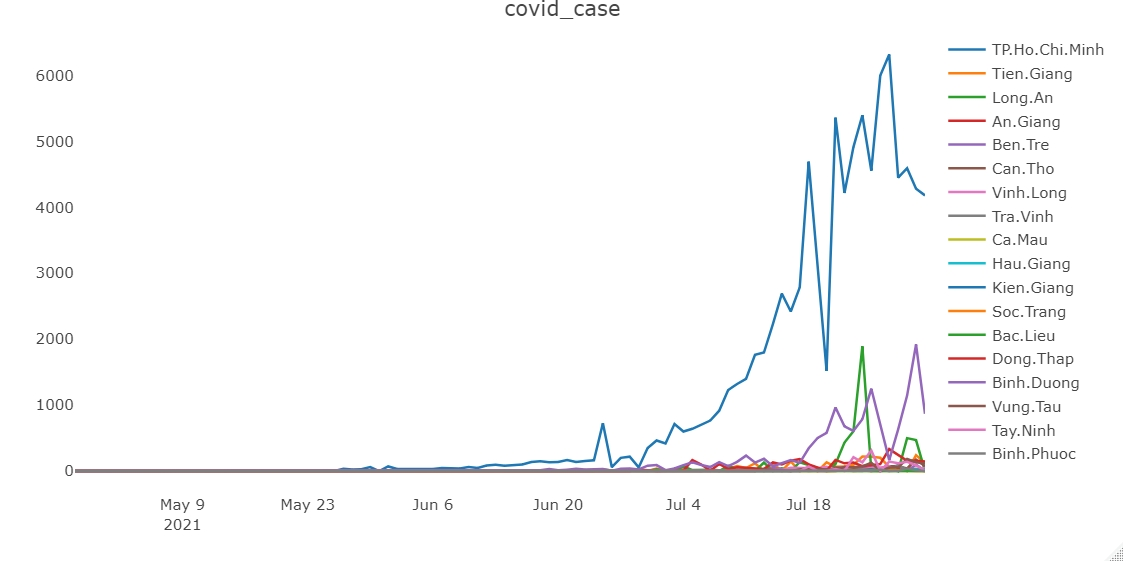
\includegraphics[width=1\linewidth]{images/Rplot01}		\label{fig:Rplot01}}
		\subfigure[Đồ thị thể hiện số lượng ca nhiễm hằng ngày tính từ ngày 27/4 trừ thành phố Hồ Chí Minh]{
			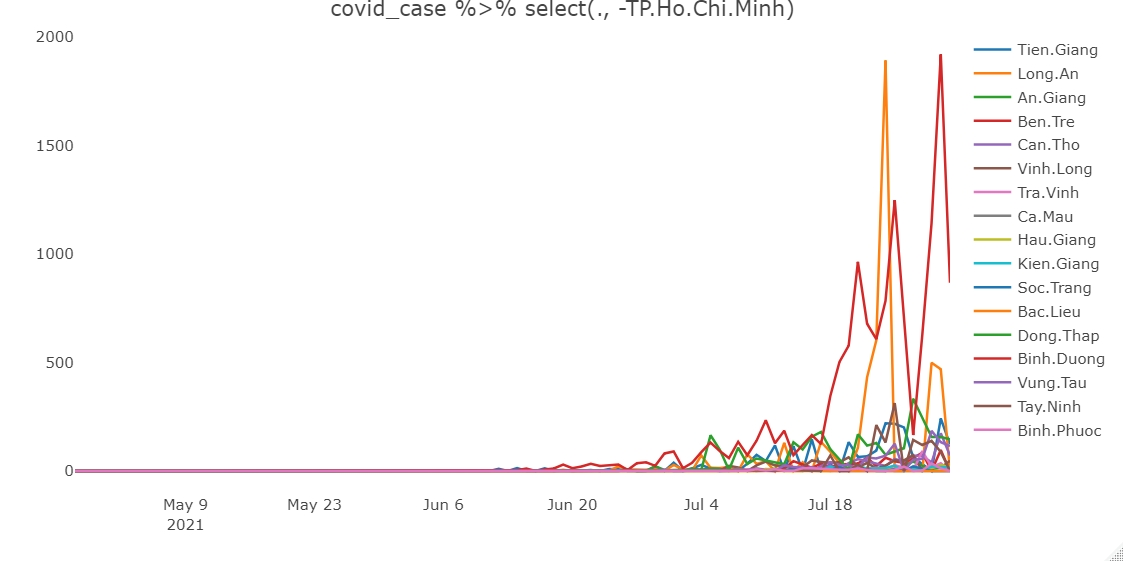
\includegraphics[width=1\linewidth]{images/Rplot02}		\label{fig:Rplot02}}
		\caption[Đồ thị số ca nhiễm hằng ngày]{Đồ thị số ca nhiễm hằng ngày. Để được tiện trong tra cứu các số liệu, chúng tôi trực quan đồ thị thể hiện số lương ca nhiễm trừ thành phố Hồ Chí Minh. Ta nhận ra có ba tỉnh/thành phố có số ca nhiễm trong ngày khá cao và khác biệt với các tỉnh/thành phố khác là Thành phố Hồ Chí Minh, Bình Dương và Long An đều nằm tập trung ở Đông Nam Bộ và đều có ranh giới với nhau. \label{fig:case}}
	\end{figure}

Khi xem xét toàn bộ dữ liệu, ta thấy các trường hợp xác nhận nhiễm bệnh ở các tỉnh phía Nam bắt đầu có dấu hiệu bùng phát từ khoảng cuối tháng năm, tức sau khi bắt đầu đợt dịch lớn ở Bắc Giang khoảng một tháng. Bắt đầu nhiễm mạnh ở thành phố Hồ Chí Minh sau đó, dịch bệnh lan rộng ra các tỉnh Đông Nam Bộ và bùng phát toàn phía Nam. 

Nhìn tổng quan đồ thị hình~\ref{fig:case}, ta nhận thấy sự khác biệt rõ ràng những ca có bệnh giữa các tỉnh. Trong đó, thành phố Hồ Chí Minh có số lượng người bệnh được xác nhận là cao nhất mỗi ngày đỉnh điểm lên đến gần 6000 ca/ngày. Các tỉnh Bình Dương và Long An cũng có xu hướng tăng mạnh vào những tuần gần đây nhất và cao nhất gần 2000 ca mắc một ngày. Các tỉnh còn lại có số ca mắc không quá cao (dưới 100 ca/ngày) nhưng vẫn có xu hướng tăng và tăng dài kỳ. 

Đồ thị tích lũy các ca xác nhận bệnh có Covid-19 thể hiện xu hướng tăng chưa có dấu hiệu đỉnh dịch. Bình Dương có số ca nhiễm bệnh cao sau thành phố Hồ Chí Minh Xu hướng tăng mạnh ở tỉnh Long An khi trong khoảng thời gian ngắn (từ ngày 21/7 đến ngày 24/7, tức 3 ngày) nhưng số ca mắc tăng đột ngột 2926 ca nhiễm. 
\begin{figure}
	\subfigure[Đồ thị thể hiện số lượng ca nhiễm tích lũy tính từ ngày 27/4]{
		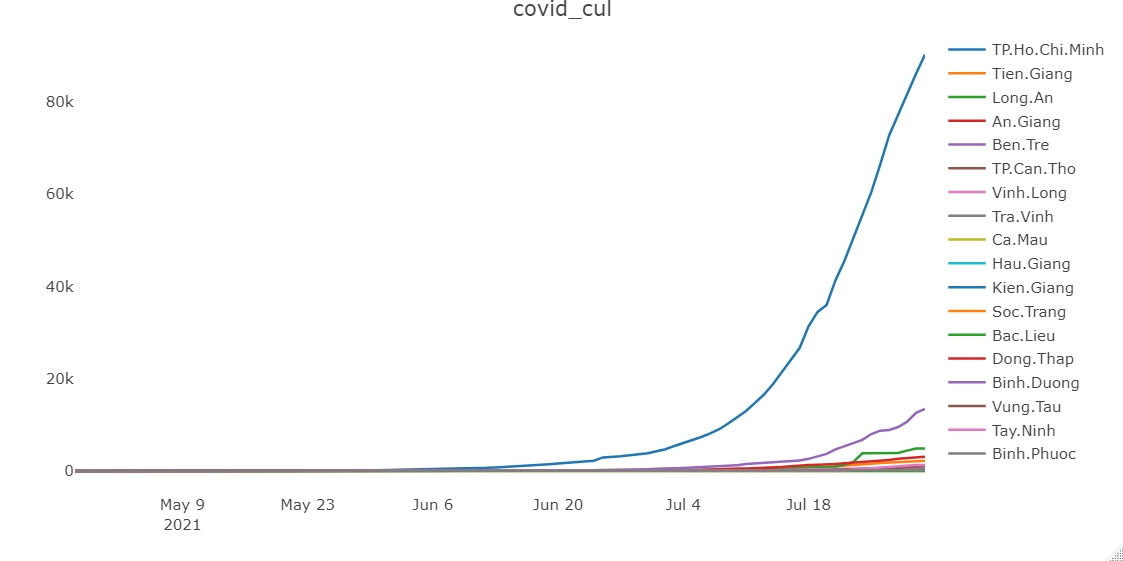
\includegraphics[width=1\linewidth]{images/Rplot03}		\label{fig:Rplot03}}
	\subfigure[Đồ thị thể hiện số lượng ca nhiễm tích lũy tính từ ngày 27/4 trừ thành phố Hồ Chí Minh]{
		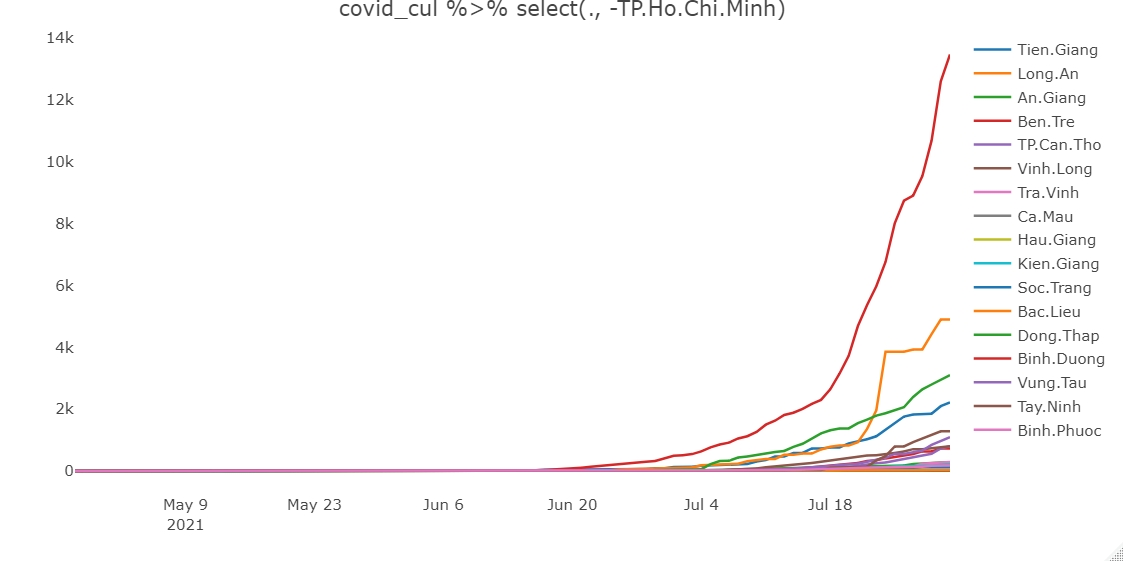
\includegraphics[width=1\linewidth]{images/Rplot04}		\label{fig:Rplot04}}
			\caption[Đồ thị số ca nhiễm tích lũy]{Đồ thị số ca nhiễm tích lũy nhằm thể hiện tốc độ tăng nhanh các ca nhiễm. Đồ thị (b) cho ta thấy tỉnh Bình Dương có xu hướng tăng sau thành phố Hồ Chí Minh. Cũng trong đồ thị (b) ta thấy rõ hơn mức độ tăng bất thường của tỉnh Long An.\label{fig:cul}}
\end{figure}





\newpage
\section{Mối tương quan đối với số ca nhiễm bệnh giữa các tỉnh}

\textbf{Đối với dữ liệu các ca nhiễm thu thập hằng ngày}, tương quan đồ dưới đây thể hiện quan hệ giữa các biến ứng với số ca nhiễm mỗi ngày. Tương quan thuận cao cho biết các biến có xu hướng đồng biến giữa hai cặp biến và nhằm dự báo xu hướng tăng trong tương lai.

\begin{Shaded}
	\begin{Highlighting}[]
\NormalTok{corrplot}\SpecialCharTok{::}\FunctionTok{corrplot.mixed}\NormalTok{(cor\_data }\OtherTok{\textless{}{-}} \NormalTok{case\_data }\SpecialCharTok{\%\textgreater{}\%} \FunctionTok{cor}\NormalTok{()}\NormalTok{, }
		\AttributeTok{tl.cex =} \FloatTok{0.5}\NormalTok{, }
		\AttributeTok{tl.col =} \StringTok{"black"}\NormalTok{, }
		\AttributeTok{order =}\StringTok{"hclust"}\NormalTok{,}
		\AttributeTok{addCoefasPercent =} \ConstantTok{TRUE}\NormalTok{,}
		\AttributeTok{upper=}\StringTok{"ellipse"}\NormalTok{)}
	\end{Highlighting}
\end{Shaded}
\begin{figure}[H]
	\centering
	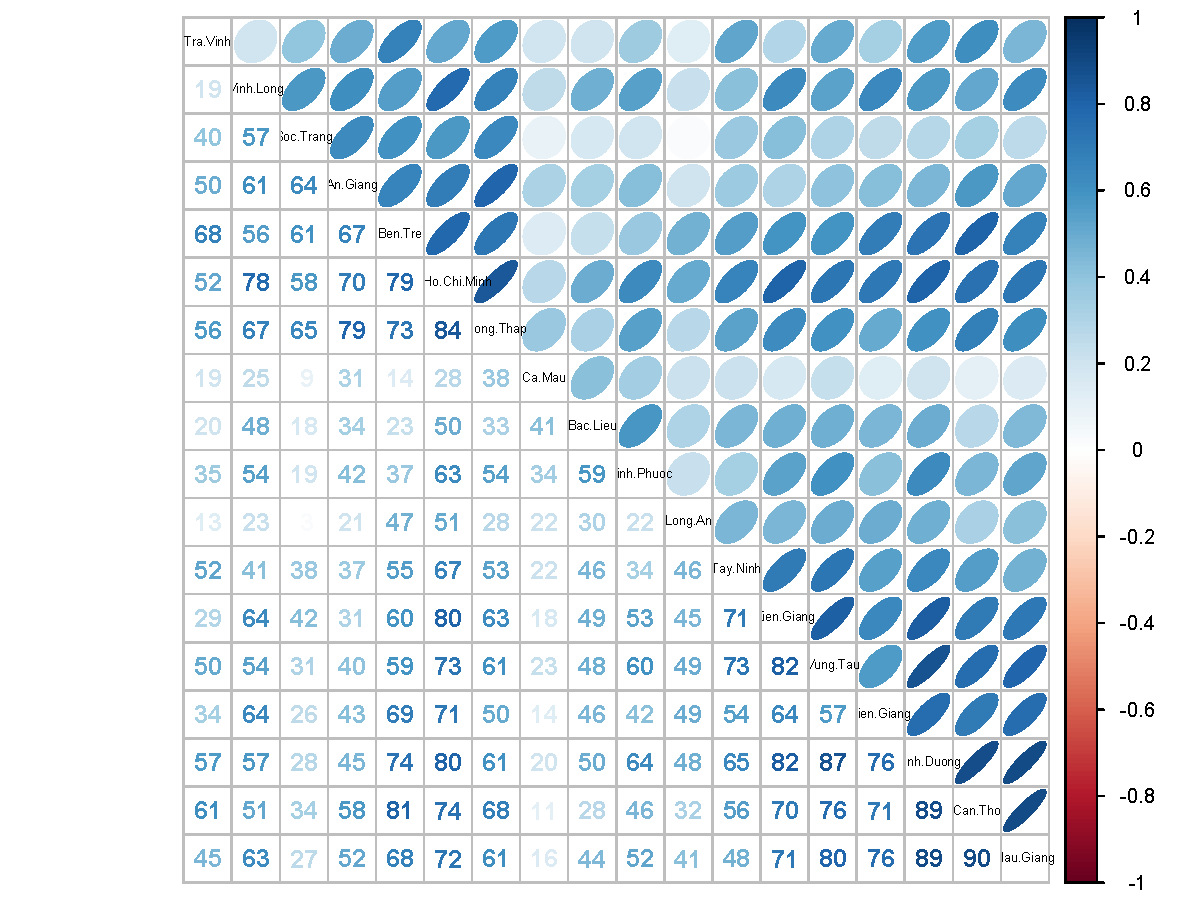
\includegraphics[width=0.8\linewidth]{images/corr_case}
	\caption[Tương quan đồ thể hiện tương quan dữ liệu hằng ngày các ca xác nhận nhiễm ở các tỉnh/thành phố.]{Tương quan đồ thể hiện tương quan dữ liệu hằng ngày các ca xác nhận nhiễm ở các tỉnh/thành phố. Trong đồ thị này, hệ số tương quan càng lớn thể hiện xu hướng tăng các ca nhiễm theo ngày càng cao giữa hai biến bất kỳ. Mức độ (độ lớn) của tương quan thể hiện bởi mức độ đậm nhạt của màu sắc được chú thích trong phổ màu bên phải.}
	\label{fig:corrcase}
\end{figure}

Qua tương quan đồ, không có một cặp biến nào có tương quan âm. Tức là mỗi ngày, dự báo về số ca nhiễm sẽ có thể tiếp tục tăng. Một số cặp tỉnh/thành phố có hệ số tương quan khá cao như Hậu Giang -- Cần Thơ ($ 90\% $), Bình Dương -- Tp. Hồ Chí Minh ($ 80\% $) hoặc Bình Dương -- Hậu Giang ($ 89\% $) là những tỉnh/thành phố có vị trí địa lý giáp nhau hoặc chịu ảnh hưởng bởi thành phố có nhiều ca bệnh.



\newpage

Từ dữ liệu tích lũy, ta có ma trận tương quan Pearson cho 18 biến phụ thuộc tạo thành tương quan đa điểm. Các hệ số tương quan trong từng cặp biến được thể hiện qua tương quan đồ.

\begin{Shaded}
	\begin{Highlighting}[]
\NormalTok{corrplot}\SpecialCharTok{::}\FunctionTok{corrplot.mixed}\NormalTok{(cor\_data }\OtherTok{\textless{}{-}} \NormalTok{cul\_data }\SpecialCharTok{\%\textgreater{}\%} \FunctionTok{cor}\NormalTok{()}\NormalTok{, }
		\AttributeTok{tl.cex =} \FloatTok{0.5}\NormalTok{, }
		\AttributeTok{tl.col =} \StringTok{"black"}\NormalTok{, }
		\AttributeTok{order =}\StringTok{"hclust"}\NormalTok{,}
		\AttributeTok{addCoefasPercent =} \ConstantTok{TRUE}\NormalTok{,}
		\AttributeTok{upper=}\StringTok{"ellipse"}\NormalTok{)}
	\end{Highlighting}
\end{Shaded}
\begin{figure}[H]
	\centering
	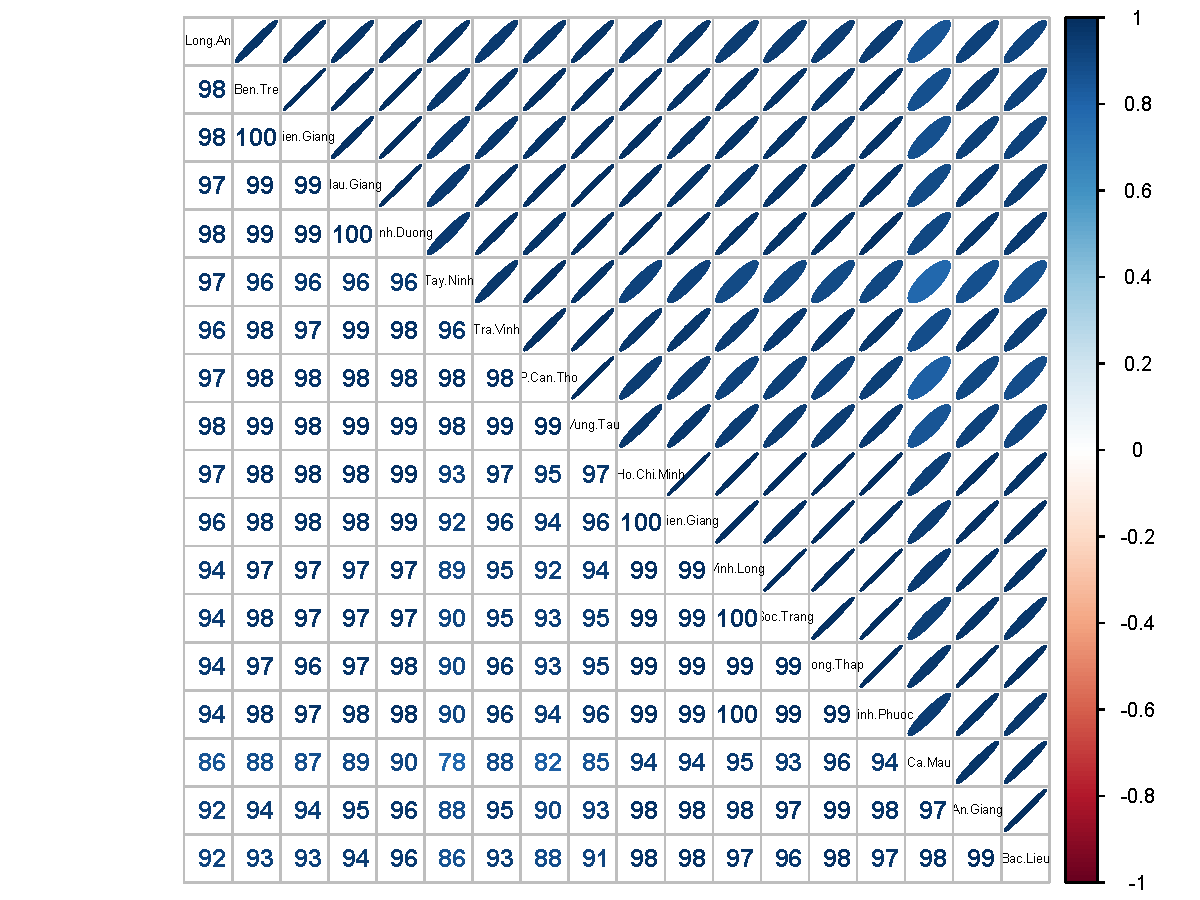
\includegraphics[width=0.8\linewidth]{images/corr_cul}
	\caption[Tương quan đồ thể hiện tương quan dữ liệu tích lũy các ca xác nhận nhiễm]{Tương quan đồ thể hiện tương quan dữ liệu tích lũy các ca xác nhận nhiễm ở các tỉnh/thành phố. Trong biểu đồ này, các số liệu thể hiện phần trăm tương quan ở mỗi biến tuân theo phổ màu; Các hình ellipse mô tả tương quan thuận ứng với số phần trăm tương quan khi diện tích càng nhỏ; Tương quan đồ đã được phân cụm và tuân theo phổ màu phía bên phải.}
	\label{fig:corrcul}
\end{figure}


Ta dễ dàng nhận thấy và cũng không quá ngạc nhiên rằng từ hình \ref{fig:corrcul} hầu hết các cặp biến tương quan thuận rất cao. Đặc biệt ở một số tỉnh tương quan chặt chẽ có hệ số tương quan gần như $ 100\% $. Một số cặp biến tương quan không quá cao như Cà Mau -- Tây Ninh ($ 78\% $) hoặc Cần Thơ -- Cà Mau ($ 82\% $) có thể được suy diễn nguyên nhân khác biệt khoảng cách địa lý và nhiều lệnh giãn cách xã hội được đặt ra nối tiếp nhau khi dịch bệnh bắt đầu bùng phát nhanh ở các tỉnh miền Nam. 







\newpage

Trong trường hợp phân tích tương quan, mối liên kết giữa 2 biến được xác lập nhờ vào giá trị của r và p-value. Ta sẽ mượn các công cụ và lý thuyết Network analysis cho mục tiêu phân tích tương quan
  \begin{Shaded}
	\begin{Highlighting}[]
\NormalTok{Graph\_pcor }\OtherTok{\textless{}{-}}\NormalTok{ case\_data }\SpecialCharTok{\%\textgreater{}\%} \FunctionTok{cor}\NormalTok{() }\SpecialCharTok{\%\textgreater{}\%} 
\NormalTok{  qgraph}\SpecialCharTok{::}\FunctionTok{qgraph}\NormalTok{(., }
		\AttributeTok{graph =} \StringTok{"pcor"}\NormalTok{, }
		\AttributeTok{layout =} \StringTok{"spring"}\NormalTok{, }
		\AttributeTok{threshold =} \StringTok{"bonferroni"}\NormalTok{,}
		\AttributeTok{sampleSize =} \FunctionTok{nrow}\NormalTok{(case\_data), }
		\AttributeTok{alpha =} \FloatTok{0.05}\NormalTok{)}
	\end{Highlighting}
\end{Shaded}

\begin{figure}[H]
	\centering
	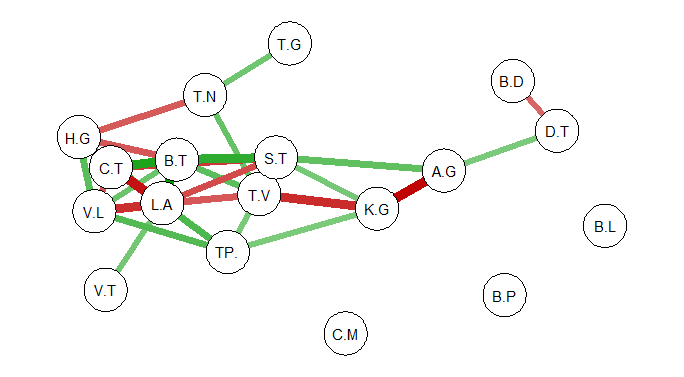
\includegraphics[width=0.7\linewidth]{images/net_case_05}
	\caption[Mạng tương quan pcor đối với dữ liệu ca bệnh thu nhập hằng ngày]{Mạng tương quan pcor đối với dữ liệu ca bệnh thu nhập hằng ngày. Đồ thị nhằm đánh giá sự tương tác giữa các biến dữ liệu qua khoảng cách các biến, độ đậm nhạt của các dây cung và màu sắc}
	\label{fig:netcase05}
\end{figure}

Từ đồ thị mạng tương quan, ta thấy rõ hơn sự tương tác giữa các tỉnh/thành phố từ dữ liệu thu thập hằng ngày. Các tỉnh tập trung thành nhóm biểu thị sự tương tác cao. Các tỉnh không có tương tác nghĩa là hệ số tương quan không có ý nghĩa thống kê với mức ý nghĩa $ 0.05 $. Độ dài và độ đậm của dây cung biểu thị mức độ tương tác cụ thể giữa các cặp biến. Tỷ lệ của các cạnh theo chiều rộng và độ bão hòa màu. Các cạnh có trọng lượng tuyệt đối lớn hơn giá trị này sẽ có cường độ màu mạnh nhất và càng rộng càng mạnh và các cạnh có trọng lượng tuyệt đối dưới giá trị này sẽ có chiều rộng nhỏ nhất và càng mờ thì trọng lượng càng yếu. Màu xanh thể hiện tương tác thuận, màu đỏ thể hiện tương tác nghịch.

Trong đồ thị mạng tương quan, cụm các biến Can.Tho, Ben.Tre, Vinh.Long, Hau.Giang tương tác cao với nhiều tỉnh thành khác và tương tác lẫn nhau. TP. Hồ Chí Minh tương tác thuận cao với các tỉnh Vĩnh Long, Long An, Trà Vinh và Kiên Giang. Ba biến Ca.Mau, Binh.Phuoc và Bạc Liêu tương quan không có ý nghĩa thống kê. 









\begin{Shaded}
	\begin{Highlighting}[]
\NormalTok{Graph\_pcor }\OtherTok{\textless{}{-}}\NormalTok{ cul\_data }\SpecialCharTok{\%\textgreater{}\%} \FunctionTok{cor}\NormalTok{() }\SpecialCharTok{\%\textgreater{}\%} 
\NormalTok{  qgraph}\SpecialCharTok{::}\FunctionTok{qgraph}\NormalTok{(., }
		\AttributeTok{graph =} \StringTok{"pcor"}\NormalTok{, }
		\AttributeTok{layout =} \StringTok{"spring"}\NormalTok{, }
		\AttributeTok{threshold =} \StringTok{"bonferroni"}\NormalTok{,}
		\AttributeTok{sampleSize =} \FunctionTok{nrow}\NormalTok{(cul\_data), }
		\AttributeTok{alpha =} \FloatTok{0.05}\NormalTok{)}
	\end{Highlighting}
\end{Shaded}

\begin{figure}[H]
	\centering
	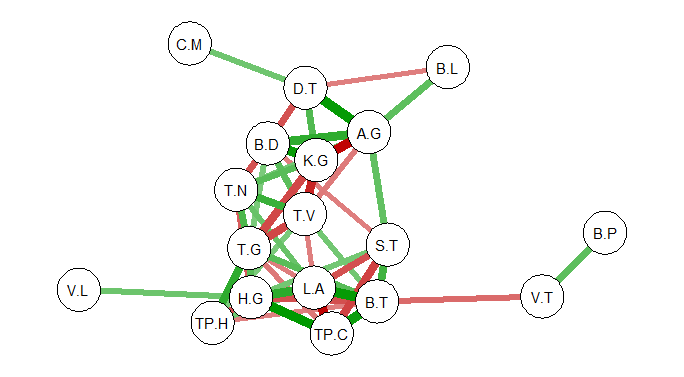
\includegraphics[width=0.7\linewidth]{images/net_cul_05}
	\caption[Mạng tương quan pcor đối với dữ liệu ca bệnh tích lũy hằng ngày]{Mạng tương quan pcor đối với dữ liệu ca bệnh tích lũy hằng ngày.}
	\label{fig:netcul05}
\end{figure}

Trong đồ thị mạng tương quan trên, tất cả các biến đều có sự tương quan tập trung. 

\begin{figure}[H]
	\centering
	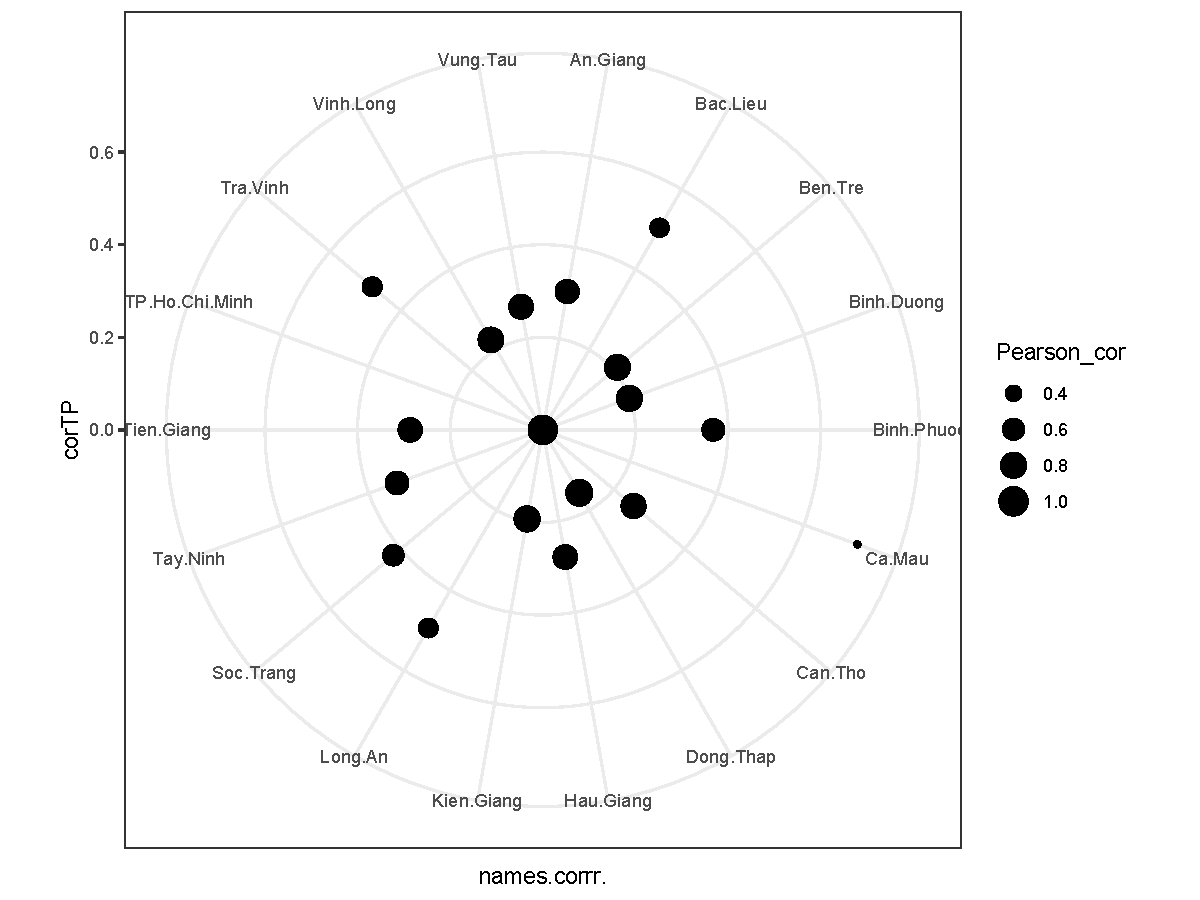
\includegraphics[width=0.7\linewidth]{images/Pearson}
	\caption[Biểu đồ tương quan giữa Thành phố Hồ Chí Minh và các tỉnh lân cận]{Biểu đồ tương quan giữa Thành phố Hồ Chí Minh và các tỉnh lân cận. Biểu đồ thể hiện mối tương quan Pearson giữa biến Tp.Ho.Chi.Minh và các biến khác trong hệ tọa độ cực. Tâm điểm của biểu đồ tương ứng với giá trị $ r=1 $ (tương quan mạnh nhất) còn ngoại vi biểu đồ tương ứng với $ r=0 $ (không có tương quan). Từ đó nhận thấy, khi càng gần về tâm biểu đồ, ta có tương quan mạnh giữa Tp. Hồ Chí Minh và ngược lại.}
	\label{fig:pearson}
\end{figure}










\newpage
\section{Phân tích thành phần chính}

Ta tiến hành thuật toán phân tích thành phần chính để chọn ra số thành phần với hy vọng phản ánh cao nhất phần trăm phương sai dữ liệu. Để dễ dàng trong phân tích, phần này chia thành hai mục phân tích riêng từng loại dữ liệu.



\subsection{Dữ liệu \textbf{\textsf{case\_data}}}
\begin{Shaded}
	\begin{Highlighting}[]
\NormalTok{case\_data }\SpecialCharTok{\%\textgreater{}\%}\NormalTok{ psych}\SpecialCharTok{::}\FunctionTok{fa.parallel}\NormalTok{(., }
		\AttributeTok{main =} \StringTok{"Scree plot with parallel analysis"}\NormalTok{)}
	\end{Highlighting}
\end{Shaded}

\begin{verbatim}
## Parallel analysis suggests that the number of factors =  3  and the number of 
## components =  1
\end{verbatim}

\begin{figure}[H]
	\centering
	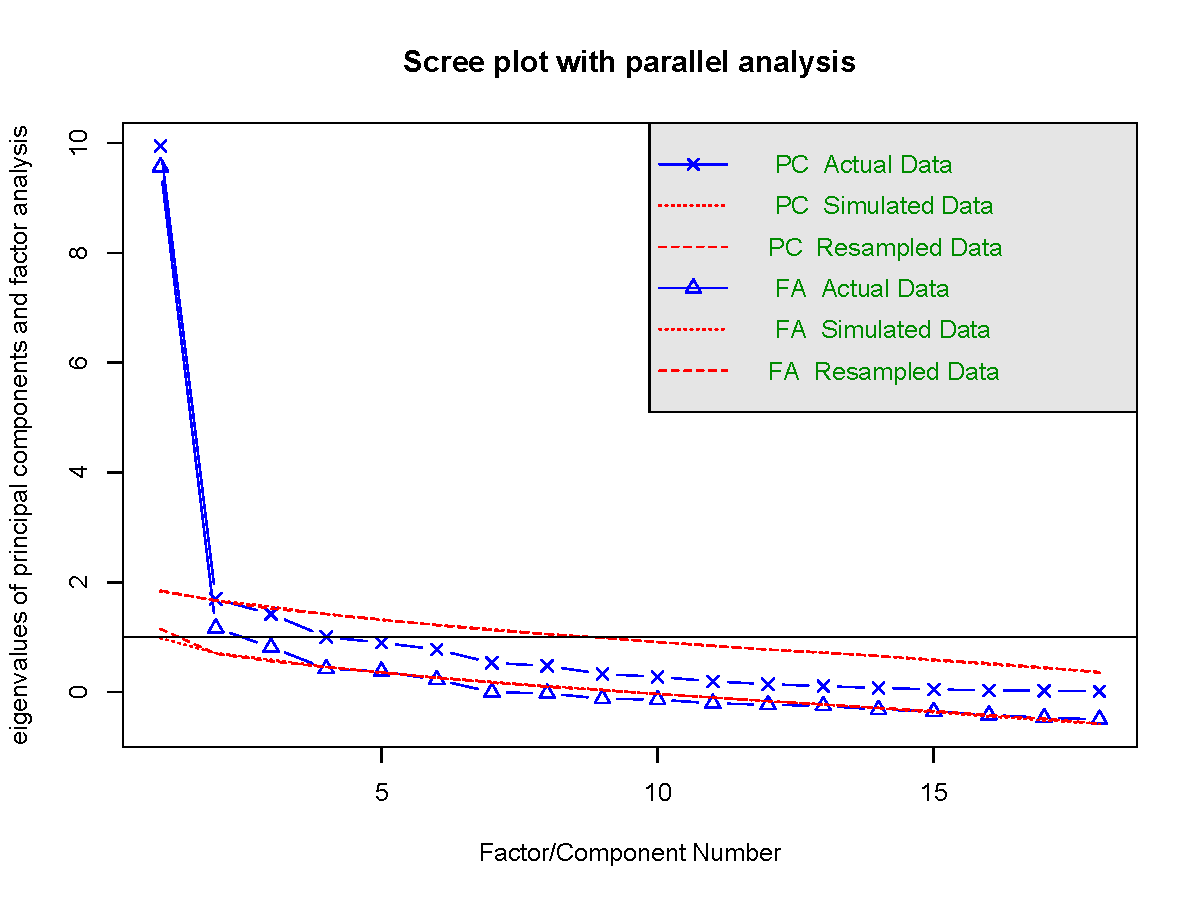
\includegraphics[width=1\linewidth]{images/scree_parall}
	\caption[Sơ đồ sàng lọc với phân tích song song dữ liệu ca nhiễm hằng ngày]{Sơ đồ sàng lọc với phân tích song song dữ liệu ca nhiễm hằng ngày. Sơ đồ cũng đề nghị số thành phần là 1 và số nhân tố là 3. Đường vạch đen thể hiện ngưỡng giá trị riêng $ 1.0 $ theo tiêu chuẩn chọn các thành phần chính. }
	\label{fig:screeparall}
\end{figure}

Qua sơ đồ sàng lọc giữa số thành phần chính và các giá trị riêng khi phân tích thành phần, ta thấy số thành phần có giá trị riêng lớn hơn $ 1 $ là 2 thành phần. Để có thể tính toán chính xác giá trị của các giá trị riêng, bài báo cáo sẽ để ở phần phân tích tiếp theo. Ngoài ra phân tích trong lệnh này cũng cho ta gợi ý lựa chọn số các nhân tố sẽ hữu dụng khi phân tích nhân tố cũng như số thành phần chính. 

Ta chọn số thành phần là nhiều hơn hai (thành phần) với mục tiêu tìm được trên $ 60\% $ tổng phương sai. Khi đó các thành phần chính sẽ giải thích được tương đối đầy đủ dữ liệu.

Tiếp theo ta xem xét các giá trị độ lệch chuẩn\index{độ lệch chuẩn}, phần trăm phương sai\index{phần trăm phương sai} cũng như phần trăm phương sai tích luỹ\index{phần trăm phương sai tích luỹ} sau khi dùng lệnh \textbf{prcomp} có sẵn trong R để phân tích thành phần chính.

\begin{Shaded}
	\begin{Highlighting}[]
\FunctionTok{prcomp}\NormalTok{(case\_data,} \AttributeTok{center =} \ConstantTok{TRUE}\NormalTok{, }\AttributeTok{scale =} \ConstantTok{TRUE}\NormalTok{) }\SpecialCharTok{\%\textgreater{}\%} 
	\FunctionTok{summary}\NormalTok{()}
	\end{Highlighting}
\end{Shaded}

\begin{verbatim}
## Importance of components:
##                           PC1     PC2     PC3     PC4     PC5    PC6     PC7
## Standard deviation     3.1537 1.30172 1.19334 1.00157 0.94887 0.8808 0.72960
## Proportion of Variance 0.5525 0.09414 0.07911 0.05573 0.05002 0.0431 0.02957
## Cumulative Proportion  0.5525 0.64667 0.72578 0.78151 0.83153 0.8746 0.90420
##                            PC8     PC9    PC10    PC11   PC12    PC13    PC14
## Standard deviation     0.69075 0.57371 0.52808 0.44200 0.3796 0.32740 0.27600
## Proportion of Variance 0.02651 0.01829 0.01549 0.01085 0.0080 0.00595 0.00423
## Cumulative Proportion  0.93071 0.94899 0.96449 0.97534 0.9833 0.98930 0.99353
##                           PC15    PC16    PC17    PC18
## Standard deviation     0.21968 0.17769 0.15258 0.11543
## Proportion of Variance 0.00268 0.00175 0.00129 0.00074
## Cumulative Proportion  0.99621 0.99797 0.99926 1.00000
\end{verbatim}


Thành phần chính đầu tiên có phần trăm phương sau giải thích $ 55.3\% $ dữ liệu. Khi thành phần chính là 2 ta thấy phần trăm tích lũy ở \textsf{PC2} đạt $ 64.7\% $. Việc giải thích được trên $ 60\% $ dữ liệu là kết quả khá tốt khi phân tích thành phần chính. Nếu ta chọn số thành phần chính là 3 thì tổng phần trăm tích lũy chỉ tăng nhẹ (khoảng $ 8\% $) và nâng việc giải thích dữ liệu khi tăng thêm một chiều thành $ 72.6\% $. 

Để tổng phần trăm phương sai trên $ 80\% $, ta chọn số thành phần chính là 5 thành phần từ 18 biến dữ liệu. Chúng tôi cũng khảo sát tỷ lệ đóng góp được trích gọn kết quả như sau

\begin{Shaded}
	\begin{Highlighting}[]
\FunctionTok{princomp}\NormalTok{(case\_data, }\AttributeTok{scores =} \ConstantTok{TRUE}\NormalTok{) }\SpecialCharTok{\%\textgreater{}\%} 
	\FunctionTok{loadings}\NormalTok{()}
	\end{Highlighting}
\end{Shaded}

\begin{verbatim}
## 
## Loadings:
##                Comp.1 Comp.2 Comp.3 Comp.4 Comp.5 Comp.6 Comp.7 Comp.8 Comp.9
## TP.Ho.Chi.Minh  0.985  0.160                                                 
## Tien.Giang                           0.563  0.436 -0.653 -0.126         0.129
## Long.An               -0.633  0.767                                          
## An.Giang                                                                     
## Ben.Tre                                           -0.166  0.481  0.419 -0.516
## Can.Tho                                           -0.166  0.255  0.586  0.351
## Vinh.Long                                                -0.408        -0.726
## Tra.Vinh                                                  0.337              
## Ca.Mau                                                                       
## Hau.Giang                                                                    
## Kien.Giang                                                                   
## Soc.Trang                                                              -0.168
## Bac.Lieu                                                                     
## Dong.Thap                           -0.516 -0.406 -0.706 -0.104 -0.223       
## Binh.Duong      0.154 -0.744 -0.634                                          
## Vung.Tau                            -0.264               -0.605  0.608  0.136
## Tay.Ninh                            -0.571  0.791         0.102 -0.110       
## Binh.Phuoc                                                                   
##                Comp.10 Comp.11 Comp.12 Comp.13 Comp.14 Comp.15 Comp.16 Comp.17
## TP.Ho.Chi.Minh                                                                
## Tien.Giang      0.152                                                         
## Long.An                                                                       
## An.Giang               -0.414  -0.755   0.277          -0.284          -0.264 
## Ben.Tre                 0.440  -0.141  -0.155   0.163           0.156         
## Can.Tho        -0.509  -0.291   0.136  -0.148  -0.119          -0.167         
## Vinh.Long      -0.277  -0.356   0.266                                         
## Tra.Vinh        0.660  -0.464   0.385          -0.185  -0.105                 
## Ca.Mau                                                 -0.597           0.783 
## Hau.Giang              -0.134           0.106  -0.291   0.225   0.889         
## Kien.Giang     -0.139   0.342   0.216          -0.510  -0.597          -0.422 
## Soc.Trang               0.183  -0.154   0.356  -0.669   0.328  -0.330   0.342 
## Bac.Lieu                                               -0.153   0.170         
## Dong.Thap                                                                     
## Binh.Duong                                                                    
## Vung.Tau        0.362   0.142                                                 
## Tay.Ninh       -0.130                                                         
## Binh.Phuoc      0.150  -0.104  -0.299  -0.854  -0.338   0.105                 
##                Comp.18
## TP.Ho.Chi.Minh        
## Tien.Giang            
## Long.An               
## An.Giang              
## Ben.Tre               
## Can.Tho               
## Vinh.Long             
## Tra.Vinh              
## Ca.Mau         -0.131 
## Hau.Giang      -0.149 
## Kien.Giang     -0.115 
## Soc.Trang             
## Bac.Lieu        0.967 
## Dong.Thap             
## Binh.Duong            
## Vung.Tau              
## Tay.Ninh              
## Binh.Phuoc            

\end{verbatim}

\newpage

Khi vẽ sơ đồ sàng lọc cụ thể cho các giá trị riêng và phần trăm phương sai trích, ta có số chiều có sự phân hóa cụ thể
\begin{Shaded}
	\begin{Highlighting}[]
\NormalTok{pca\_case }\OtherTok{\textless{}{-}}\NormalTok{ FactoMineR}\SpecialCharTok{::}\FunctionTok{PCA}\NormalTok{(case\_data, }\AttributeTok{graph =} \ConstantTok{FALSE}\NormalTok{)}
\NormalTok{left }\OtherTok{\textless{}{-}}\NormalTok{ pca\_case }\SpecialCharTok{\%\textgreater{}\%}\NormalTok{ factoextra}\SpecialCharTok{::}\FunctionTok{fviz\_eig}\NormalTok{(.,}
		\AttributeTok{choice =} \StringTok{\textquotesingle{}eigenvalue\textquotesingle{}}\NormalTok{,}
		\AttributeTok{geom =} \StringTok{\textquotesingle{}line\textquotesingle{}}\NormalTok{,}
		\AttributeTok{addlabels =} \ConstantTok{TRUE}\NormalTok{,}
		\AttributeTok{repel =} \ConstantTok{TRUE}\NormalTok{)}
\NormalTok{right }\OtherTok{\textless{}{-}}\NormalTok{ pca\_case }\SpecialCharTok{\%\textgreater{}\%}\NormalTok{ factoextra}\SpecialCharTok{::}\FunctionTok{fviz\_screeplot}\NormalTok{(., }
		\AttributeTok{addlabels =} \ConstantTok{TRUE}\NormalTok{,}
		\AttributeTok{repel =} \ConstantTok{TRUE}\NormalTok{)}
\NormalTok{gridExtra}\SpecialCharTok{::}\FunctionTok{grid.arrange}\NormalTok{(left, right, }\AttributeTok{ncol =} \DecValTok{2}\NormalTok{)}
	\end{Highlighting}
\end{Shaded}
\begin{figure}[H]
	\centering
	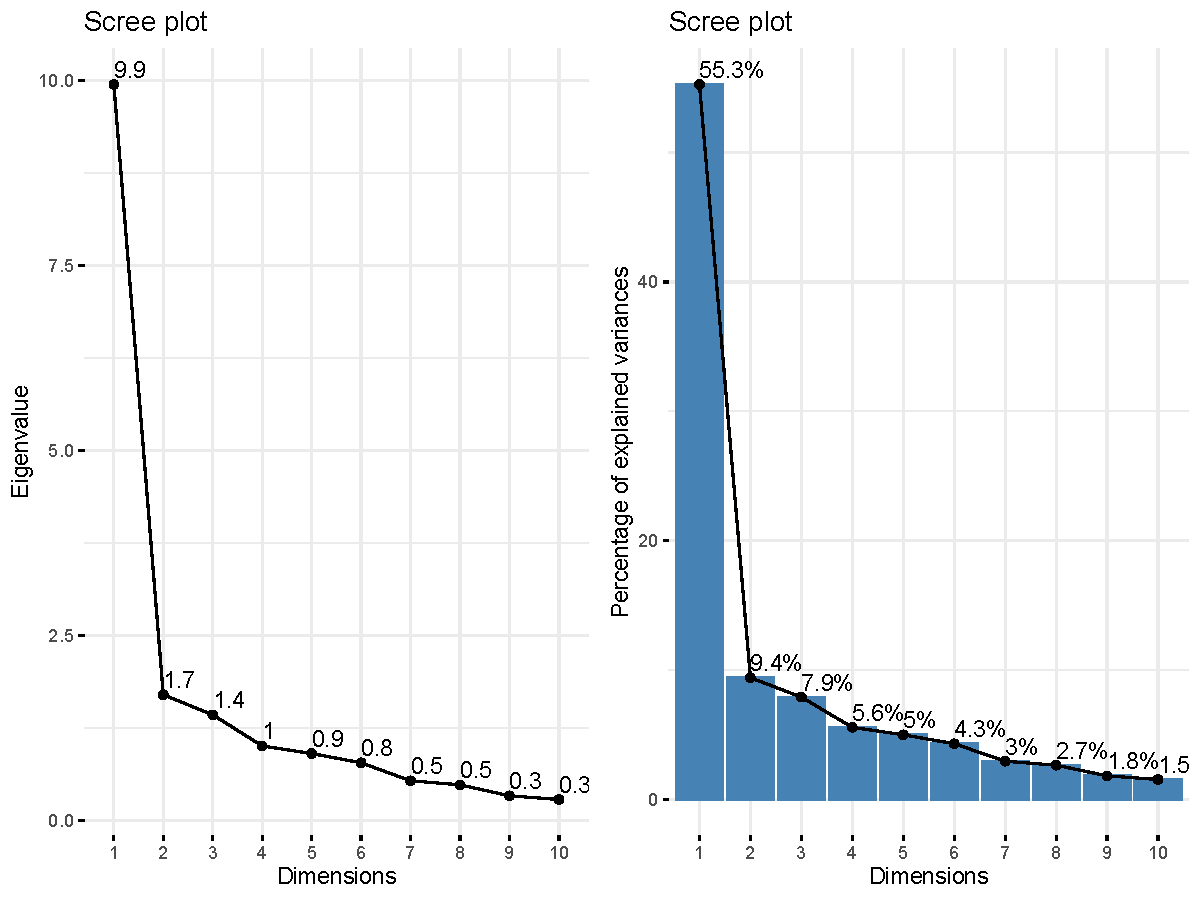
\includegraphics[width=1\linewidth]{images/Scree_plot_2}
	\caption[Sơ đồ sàng lọc dữ liệu ca nhiễm hằng ngày và giá trị riêng tương ứng]{Sơ đồ sàng lọc cho kết quả đồ thị bên trái thể hiện giá trị riêng của từng thành phần chính. Trong đồ thị này, thành phần thứ nhất có giá trị riêng lớn nhất, thành phần thứ năm trở đi thì có giá trị riêng bé hơn $ 1 $. Sơ đồ bên phải thể hiện phần trăm phương sai được giải thích đối với từng thành phần. }
	\label{fig:screeplot2}
\end{figure}

Qua sơ đồ trên, hơn $ 80\% $ các phương sai có thể được giải thích bởi chỉ $ 5 $ chiều (thành phần) đầu tiên, với thành phần thứ nhất giải thích $ 53.3\% $ như đã biết.







\newpage


Bước cuối cùng là hình dung sự phân bố của các mẫu trong không gian sắp xếp mới này, nó chỉ là một phép quay của không gian biến ban đầu của chúng ta. Điểm số mô tả vị trí của các mẫu và chúng ta vẽ biểu đồ này dưới dạng biểu đồ phân tán, bắt đầu với cặp thành phần chính quan trọng nhất (1 và 2). Lưu ý hai chiều đại diện này chỉ chiếm hơn $ 60\% $ sự giải thích dữ liệu.
\begin{Shaded}
	\begin{Highlighting}[]
\NormalTok{pca\_case }\SpecialCharTok{\%\textgreater{}\%}\NormalTok{ factoextra}\SpecialCharTok{::}\FunctionTok{fviz\_pca\_biplot}\NormalTok{(.,}
		\AttributeTok{repel =} \ConstantTok{TRUE}\NormalTok{,}
		\AttributeTok{col.var =} \StringTok{"\#2E9FDF"}\NormalTok{,}
		\AttributeTok{col.ind =} \StringTok{"\#696969"}\NormalTok{)}
	\end{Highlighting}
\end{Shaded}

\begin{figure}[H]
	\centering
	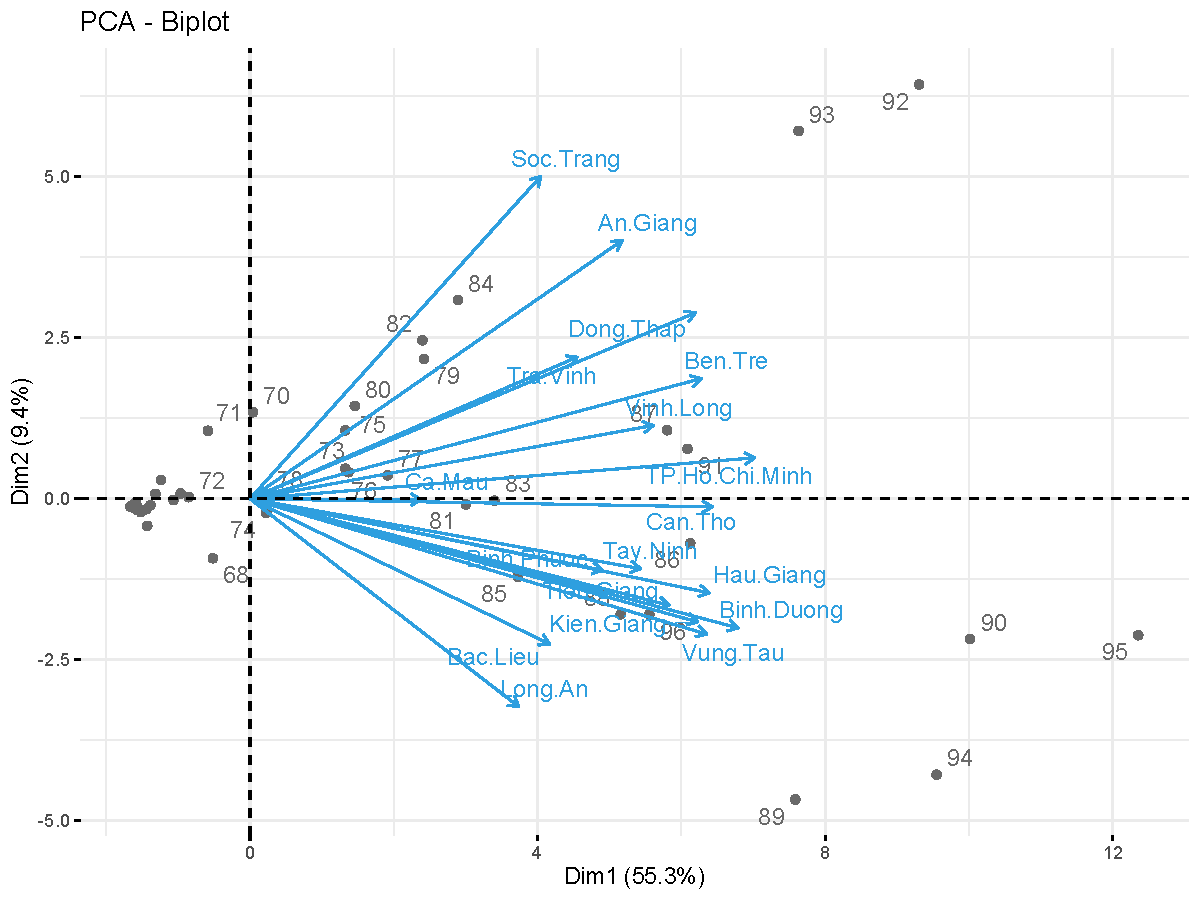
\includegraphics[width=0.7\linewidth]{images/biplot_case}
	\caption[Biểu đồ biplot cho dữ liệu hằng ngày]{Biểu đồ biplot cho biết mối quan hệ giữa các biến ban đầu và các thành phần chính. Đây được gọi là biểu đồ khoảng cách và nó hiển thị các quan sát riêng lẻ cũng như các véc-tơ tương ứng với tải. Độ dài của vector cho biết độ mạnh của mối tương quan của biến ban đầu với thành phần chính.}
	\label{fig:biplotcase}
\end{figure}

Biểu đồ cho biết vị trí các ngày được đánh số thứ tự tăng dần đến ngày thứ $ 96 $ khi chỉ sử dụng hai thành phần chính làm hệ trục tọa độ. Ngoài ra, biểu đồ biplot cũng chiếu các biến lên hệ trục tọa độ. 




\begin{Shaded}
	\begin{Highlighting}[]
\NormalTok{pca\_case }\SpecialCharTok{\%\textgreater{}\%} \FunctionTok{fviz\_pca\_ind}\NormalTok{(.,}
		\AttributeTok{col.ind =} \StringTok{"cos2"}\NormalTok{,}
		\AttributeTok{pointsize =} \StringTok{"cos2"}\NormalTok{,}
		\AttributeTok{gradient.cols =} \FunctionTok{c}\NormalTok{(}\StringTok{"\#00AFBB"}\NormalTok{, }\StringTok{"\#E7B800"}\NormalTok{, }\StringTok{"\#FC4E07"}\NormalTok{),}
		\AttributeTok{repel =} \ConstantTok{TRUE}\NormalTok{) }
	\end{Highlighting}
\end{Shaded}


\begin{figure}[H]
	\centering
	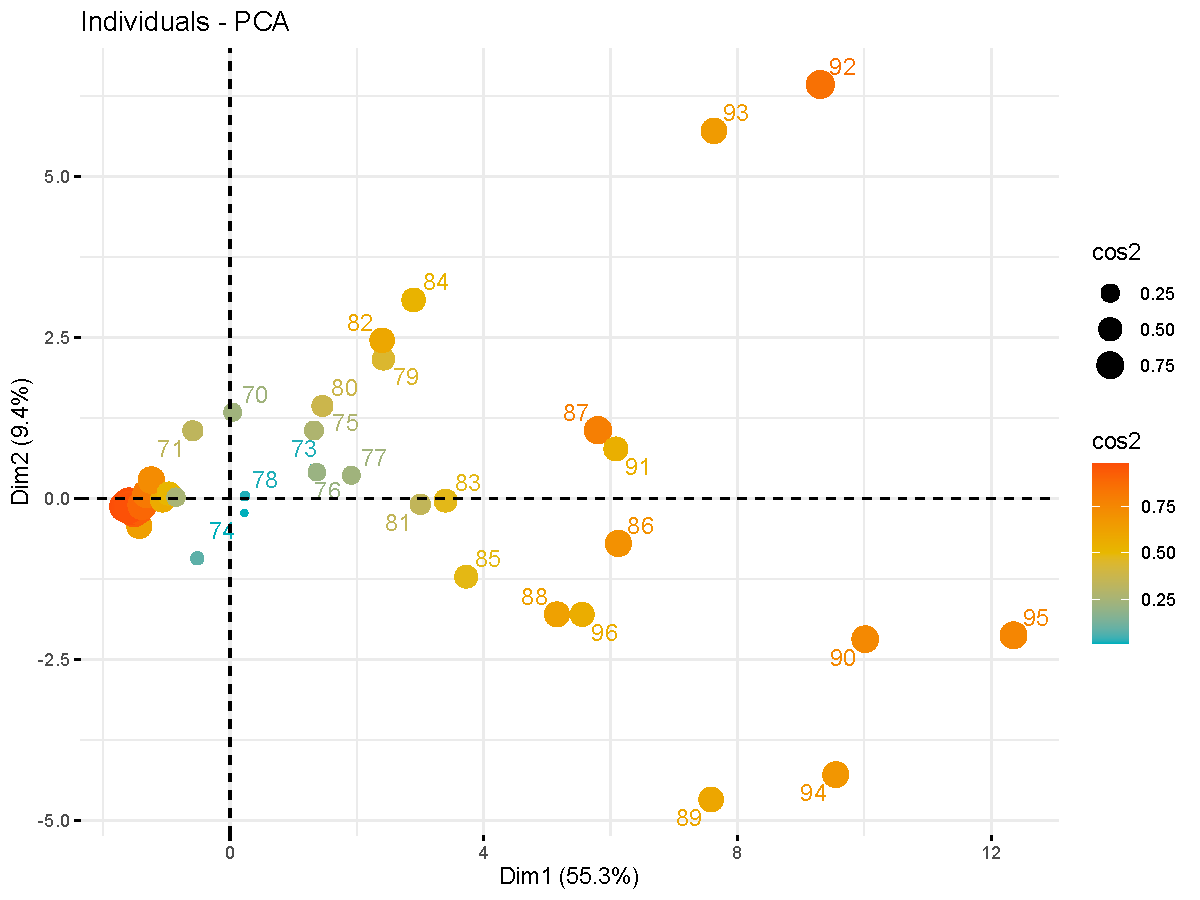
\includegraphics[width=0.7 \linewidth]{images/ind_case}
	\caption[Biểu đồ biplot tổng hợp mật độ cos2 giữa hai thành phần chính của dữ liệu hằng ngày]{Biểu đồ biplot tổng hợp mật độ cos2 giữa hai thành phần chính của dữ liệu hằng ngày. Biểu đồ giải thích chính xác hơn độ lớn của giá trị cos2 qua kích thước và phổ màu.}
	\label{fig:indcase}
\end{figure}


Biểu đồ biplot cá thể trên hai trục chính đầu tiên được thể hiện thông qua hai trục thành phần chính đầu tiên. Các giá trị cos2 (Cô-sin bình phương) càng cao thể hiện khả năng đóng góp vào thành phần chính càng cao. Ta thấy kể từ ngày thứ 71 trở đi, dữ liệu tán xạ ra hai phía của trục chính và có hệ số cos2 tăng đáng kể.

Để nói thêm về hệ số cos2 và chọn ra 5 contrib chứa đóng góp (tính theo phần trăm) của các biến cho các thành phần chính, ta tiến hành trực quan dữ liệu qua hai chiều đầu tiên trong hệ trục cực tọa độ.

\begin{Shaded}
	\begin{Highlighting}[]
\NormalTok{pca\_case }\SpecialCharTok{\%\textgreater{}\%}\NormalTok{ FactoMineR}\SpecialCharTok{::}\FunctionTok{plot.PCA}\NormalTok{(., }
		\AttributeTok{choix=}\StringTok{\textquotesingle{}var\textquotesingle{}}\NormalTok{,}
		\AttributeTok{select=}\StringTok{\textquotesingle{}contrib 5\textquotesingle{}}\NormalTok{)}
\NormalTok{pca\_case }\SpecialCharTok{\%\textgreater{}\%}\NormalTok{ factoextra}\SpecialCharTok{::}\FunctionTok{fviz\_pca\_var}\NormalTok{(., }
		\AttributeTok{col.var =} \StringTok{"cos2"}\NormalTok{,}
		\AttributeTok{gradient.cols =} \FunctionTok{c}\NormalTok{(}\StringTok{"\#00AFBB"}\NormalTok{, }\StringTok{"\#E7B800"}\NormalTok{, }\StringTok{"\#FC4E07"}\NormalTok{), }
		\AttributeTok{repel =} \ConstantTok{TRUE}\NormalTok{)}
	\end{Highlighting}
\end{Shaded}
\begin{landscape}
		\begin{figure}[H]
		\centering
		\subfigure[Đồ thị biểu diễn tương quan theo hai chiều dữ liệu đầu tiên của dữ liệu theo ngày] {
			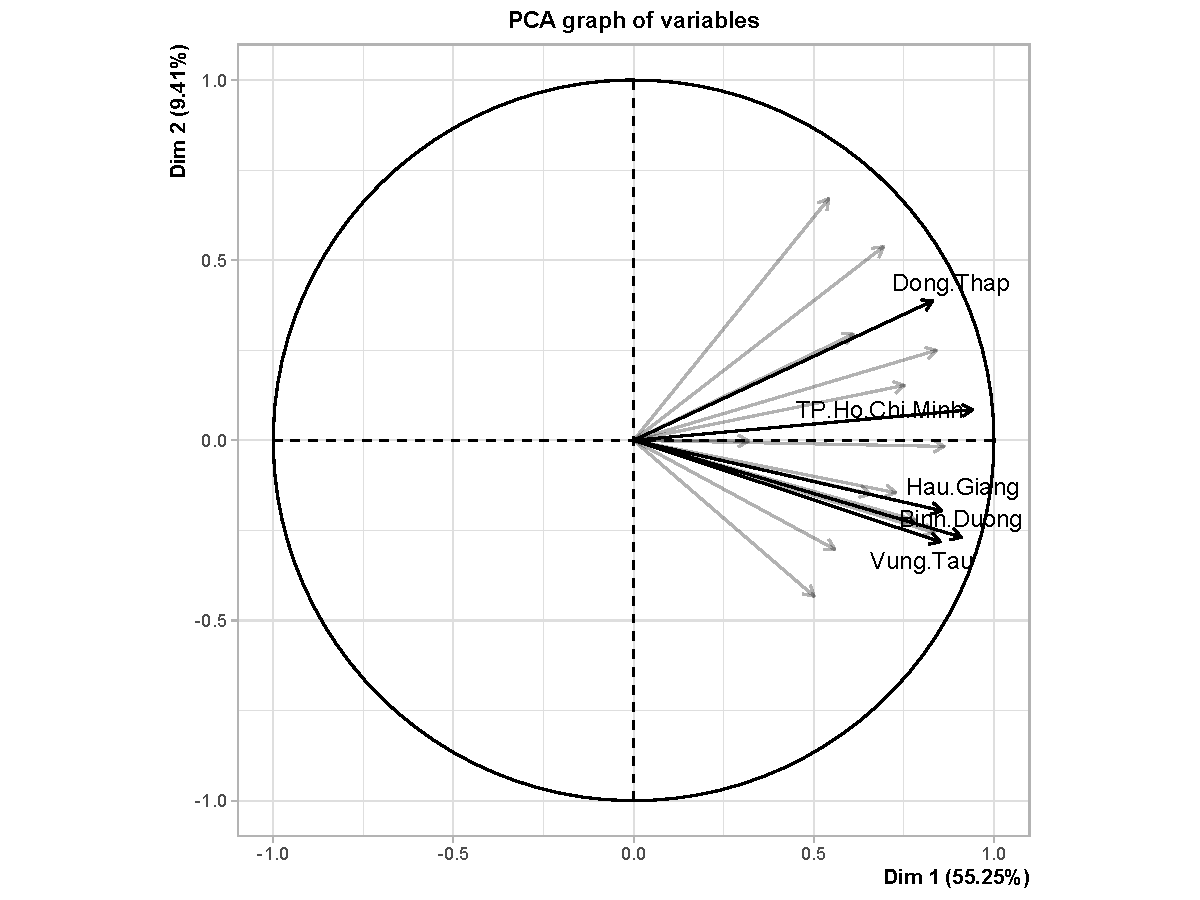
\includegraphics[width=0.48 \linewidth]{images/contrib5_case}		\label{fig:circclustcase}}
		\subfigure[Đồ thị biểu diễn cos2 của giá trị riêng theo hai chiều dữ liệu đầu tiên của dữ liệu theo ngày]{
			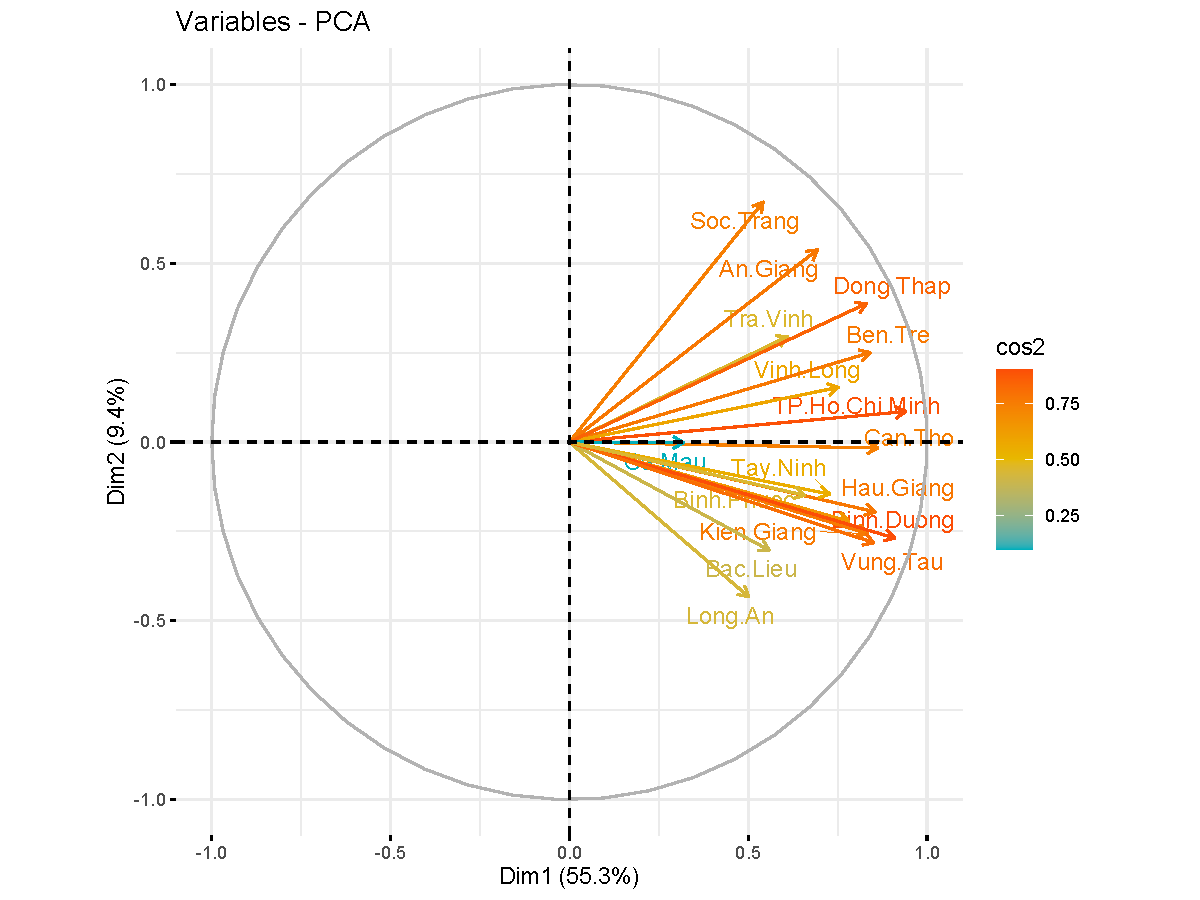
\includegraphics[width=0.48\linewidth]{images/circ_cos2_case}		\label{fig:circcos2case}}
		\caption{Đồ thị biểu diễn các thông số theo hai chiều dữ liệu đầu tiên.}
	\end{figure}

Dựa vào biểu đồ (a) ta thấy sự khác biệt hệ số tải giữa các thành phần chính. Các biến có tương quan thuận được nhóm lại với nhau. Tất cả các biến đều có tương quan thuận khi xét thành phần thứ nhất và khi xét thành phần thứ hai, các biến được chia thành hai nhóm có tương quan âm và dương. Khi chọn số thành phần chính là 5 thành phần, ta có các thành phần chính được chia thành hai nhóm. Nhóm 1 gồm TP. Hồ Chí Minh và tỉnh Đồng Tháp có hệ số tương quan dương đối với hai chiều dữ liệu; Nhóm 2 gồm ba tỉnh Hậu Giang, Bình Dương, Vũng Tàu có hệ số tương quan ở chiều thứ nhất là hệ số dương và chiều thứ hai âm. 

Đồ thị của dữ liệu (b) cho thấy giá trị cos2\index{giá trị cos2} cao và mật độ dày đặc nằm ở bên phải trục chính thứ nhất và chia thành hai phần khi chiếu đến thành phần thứ hai. Tỉnh Sóc Trăng và Long An có xu hướng trực giao. Tp. Cần Thơ có vị trí tương quan rất cao đối với thành phần thứ nhất mà gần như không tương quan khi xét thành phần thứ hai. Qua đồ thị (a) và (b) ta có thể chọn ra 5 biến có cos2 cao nhất làm các thành phần chính và giảm chiều dữ liệu dựa trên 5 biến này. 
	
\end{landscape}



Ta có các giá trị riêng và phần trăm phương sai và phần trăm phương sai tích lũy được viết gọn theo thứ tự giảm dần các giá trị riêng cũng như tăng dần phần trăm phương sai tích lũy như sau
\begin{Shaded}
	\begin{Highlighting}[]
\NormalTok{factoextra}\SpecialCharTok{::}\FunctionTok{get\_eig}\NormalTok{(pca\_case)}
	\end{Highlighting}
\end{Shaded}
\begin{verbatim}
##        eigenvalue variance.percent cumulative.variance.percent
## Dim.1  9.94554139      55.25300770                    55.25301
## Dim.2  1.69446623       9.41370128                    64.66671
## Dim.3  1.42405017       7.91138981                    72.57810
## Dim.4  1.00313508       5.57297266                    78.15107
## Dim.5  0.90036068       5.00200375                    83.15308
## Dim.6  0.77572770       4.30959832                    87.46267
## Dim.7  0.53232157       2.95734207                    90.42002
## Dim.8  0.47713645       2.65075808                    93.07077
## Dim.9  0.32914826       1.82860147                    94.89938
## Dim.10 0.27886842       1.54926898                    96.44864
## Dim.11 0.19536717       1.08537314                    97.53402
## Dim.12 0.14407396       0.80041086                    98.33443
## Dim.13 0.10718923       0.59549572                    98.92992
## Dim.14 0.07617433       0.42319071                    99.35311
## Dim.15 0.04825925       0.26810696                    99.62122
## Dim.16 0.03157511       0.17541728                    99.79664
## Dim.17 0.02328171       0.12934282                    99.92598
## Dim.18 0.01332331       0.07401838                   100.00000
\end{verbatim}

Ta quan tâm đến 10 giá trị cá thể đầu tiên được tính toán các hệ số ctr và cos2 cho từng cá thể.

\begin{Shaded}
	\begin{Highlighting}[]
\FunctionTok{summary}\NormalTok{(pca\_case)}
	\end{Highlighting}
\end{Shaded}

\begin{verbatim}
##
## Call:
## FactoMineR::PCA(X = case_data) 
## 
## 
## Eigenvalues
##                        Dim.1   Dim.2   Dim.3   Dim.4   Dim.5   Dim.6   Dim.7
## Variance               9.946   1.694   1.424   1.003   0.900   0.776   0.532
## % of var.             55.253   9.414   7.911   5.573   5.002   4.310   2.957
## Cumulative % of var.  55.253  64.667  72.578  78.151  83.153  87.463  90.420
##                        Dim.8   Dim.9  Dim.10  Dim.11  Dim.12  Dim.13  Dim.14
## Variance               0.477   0.329   0.279   0.195   0.144   0.107   0.076
## % of var.              2.651   1.829   1.549   1.085   0.800   0.595   0.423
## Cumulative % of var.  93.071  94.899  96.449  97.534  98.334  98.930  99.353
##                       Dim.15  Dim.16  Dim.17  Dim.18
## Variance               0.048   0.032   0.023   0.013
## % of var.              0.268   0.175   0.129   0.074
## Cumulative % of var.  99.621  99.797  99.926 100.000
## 
## Individuals (the 10 first)
##                    Dist    Dim.1    ctr   cos2    Dim.2    ctr   cos2    Dim.3
## 1              |  1.689 | -1.663  0.290  0.969 | -0.122  0.009  0.005 | -0.221
## 2              |  1.689 | -1.663  0.290  0.969 | -0.122  0.009  0.005 | -0.221
## 3              |  1.689 | -1.662  0.289  0.969 | -0.122  0.009  0.005 | -0.221
## 4              |  1.689 | -1.663  0.290  0.969 | -0.122  0.009  0.005 | -0.221
## 5              |  1.689 | -1.663  0.290  0.969 | -0.122  0.009  0.005 | -0.221
## 6              |  1.689 | -1.663  0.290  0.969 | -0.122  0.009  0.005 | -0.221
## 7              |  1.689 | -1.663  0.290  0.969 | -0.122  0.009  0.005 | -0.221
## 8              |  1.689 | -1.663  0.290  0.969 | -0.122  0.009  0.005 | -0.221
## 9              |  1.689 | -1.663  0.290  0.969 | -0.122  0.009  0.005 | -0.221
## 10             |  1.689 | -1.663  0.290  0.969 | -0.122  0.009  0.005 | -0.221
##                   ctr   cos2  
## 1               0.036  0.017 |
## 2               0.036  0.017 |
## 3               0.036  0.017 |
## 4               0.036  0.017 |
## 5               0.036  0.017 |
## 6               0.036  0.017 |
## 7               0.036  0.017 |
## 8               0.036  0.017 |
## 9               0.036  0.017 |
## 10              0.036  0.017 |
## 
## Variables (the 10 first)
##                   Dim.1    ctr   cos2    Dim.2    ctr   cos2    Dim.3    ctr
## TP.Ho.Chi.Minh |  0.940  8.893  0.885 |  0.085  0.429  0.007 |  0.057  0.227
## Tien.Giang     |  0.781  6.125  0.609 | -0.221  2.892  0.049 | -0.140  1.382
## Long.An        |  0.501  2.522  0.251 | -0.432 11.036  0.187 | -0.053  0.199
## An.Giang       |  0.693  4.832  0.481 |  0.537 17.038  0.289 |  0.161  1.822
## Ben.Tre        |  0.840  7.103  0.706 |  0.250  3.686  0.062 | -0.298  6.239
## Can.Tho        |  0.862  7.464  0.742 | -0.017  0.017  0.000 | -0.350  8.585
## Vinh.Long      |  0.751  5.674  0.564 |  0.153  1.374  0.023 |  0.262  4.811
## Tra.Vinh       |  0.609  3.732  0.371 |  0.295  5.122  0.087 | -0.237  3.938
## Ca.Mau         |  0.319  1.024  0.102 | -0.002  0.000  0.000 |  0.689 33.352
## Hau.Giang      |  0.855  7.356  0.732 | -0.196  2.256  0.038 | -0.177  2.207
##                  cos2  
## TP.Ho.Chi.Minh  0.003 |
## Tien.Giang      0.020 |
## Long.An         0.003 |
## An.Giang        0.026 |
## Ben.Tre         0.089 |
## Can.Tho         0.122 |
## Vinh.Long       0.069 |
## Tra.Vinh        0.056 |
## Ca.Mau          0.475 |
## Hau.Giang       0.031 |
\end{verbatim}


\newpage
\subsection{Dữ liệu \textbf{\textsf{cul\_data}}}

Tương tự đối với dữ liệu ca bệnh tích lũy, ta cũng có sơ đồ sàng lọc và phân tích song song ca nhiễm tích lũy.
\begin{Shaded}
	\begin{Highlighting}[]
\NormalTok{cul\_data }\SpecialCharTok{\%\textgreater{}\%}\NormalTok{ psych}\SpecialCharTok{::}\FunctionTok{fa.parallel}\NormalTok{(., }
		\AttributeTok{main =} \StringTok{"Scree plot with parallel analysis"}\NormalTok{)}
	\end{Highlighting}
\end{Shaded}



\begin{figure}[H]
	\centering
	\includegraphics[width=1\linewidth]{images/scree_parallcul}
	\caption[Sơ đồ sàng lọc với phân tích song song dữ liệu ca nhiễm hằng ngày]{Sơ đồ sàng lọc với phân tích song song dữ liệu ca nhiễm tích lũy. Sơ đồ cũng đề nghị số thành phần là 1 và số nhân tố là 3. }
	\label{fig:screeparallcul}
\end{figure}

Ở đây, ta thấy kể từ thành phần chính thứ hai đã có giá trị riêng không vượt qua ngưỡng $ 1.0 $. Điều này cho thấy sự nhất quán trong dữ liệu. Để có cái nhìn đối sánh hơn, ta tiến hành phân tích thành phần chính và tìm số phần trăm giải thích phương sai thích hợp đê giải thích dữ liệu.



\newpage
\begin{Shaded}
	\begin{Highlighting}[]
\FunctionTok{prcomp}\NormalTok{(cul\_data,} \AttributeTok{center =} \ConstantTok{TRUE}\NormalTok{, }\AttributeTok{scale =} \ConstantTok{TRUE}\NormalTok{) }\SpecialCharTok{\%\textgreater{}\%} 
		\FunctionTok{summary}\NormalTok{()}
	\end{Highlighting}
\end{Shaded}

\begin{verbatim}
## Importance of components:
##                           PC1     PC2     PC3     PC4     PC5     PC6     PC7
## Standard deviation     4.1577 0.70565 0.29500 0.24320 0.14515 0.13135 0.08728
## Proportion of Variance 0.9604 0.02766 0.00483 0.00329 0.00117 0.00096 0.00042
## Cumulative Proportion  0.9604 0.98801 0.99284 0.99613 0.99730 0.99826 0.99868
##                            PC8     PC9    PC10    PC11    PC12    PC13    PC14
## Standard deviation     0.07794 0.06992 0.06559 0.05729 0.04386 0.03259 0.02960
## Proportion of Variance 0.00034 0.00027 0.00024 0.00018 0.00011 0.00006 0.00005
## Cumulative Proportion  0.99902 0.99929 0.99953 0.99971 0.99982 0.99988 0.99993
##                           PC15    PC16    PC17    PC18
## Standard deviation     0.02321 0.02225 0.01241 0.01149
## Proportion of Variance 0.00003 0.00003 0.00001 0.00001
## Cumulative Proportion  0.99996 0.99998 0.99999 1.00000
\end{verbatim}



\begin{Shaded}
	\begin{Highlighting}[]
\FunctionTok{princomp}\NormalTok{(cul\_data, }\AttributeTok{scores =} \ConstantTok{TRUE}\NormalTok{) }\SpecialCharTok{\%\textgreater{}\%} 
		\FunctionTok{loadings}\NormalTok{()}
	\end{Highlighting}
\end{Shaded}


\begin{verbatim}
##
## Loadings:
##                Comp.1 Comp.2 Comp.3 Comp.4 Comp.5 Comp.6 Comp.7 Comp.8 Comp.9
## TP.Ho.Chi.Minh  0.989  0.129                                                 
## Tien.Giang                          -0.250  0.217 -0.844 -0.376  0.153       
## Long.An               -0.557  0.794 -0.211                                   
## An.Giang                            -0.112        -0.116  0.198              
## Ben.Tre                              0.151 -0.190  0.187 -0.512        -0.485
## TP.Can.Tho                           0.136 -0.246        -0.262  0.400 -0.419
## Vinh.Long                                          0.119 -0.589 -0.554  0.342
## Tra.Vinh                                   -0.144                0.181       
## Ca.Mau                                                                       
## Hau.Giang                                                                    
## Kien.Giang                                               -0.132              
## Soc.Trang                                                                    
## Bac.Lieu                                                                     
## Dong.Thap              0.116 -0.121 -0.796 -0.540                            
## Binh.Duong      0.129 -0.772 -0.582 -0.109  0.157                            
## Vung.Tau              -0.103               -0.295        -0.236  0.571  0.659
## Tay.Ninh              -0.200         0.421 -0.654 -0.433  0.174 -0.346       
## Binh.Phuoc                                               -0.104         0.126
##                Comp.10 Comp.11 Comp.12 Comp.13 Comp.14 Comp.15 Comp.16 Comp.17
## TP.Ho.Chi.Minh                                                                
## Tien.Giang                                                                    
## Long.An                                                                       
## An.Giang        0.497   0.288  -0.673   0.231                  -0.232   0.142 
## Ben.Tre                -0.494  -0.320                   0.112           0.153 
## TP.Can.Tho              0.646   0.182                          -0.102  -0.167 
## Vinh.Long       0.242   0.309   0.103           0.197                         
## Tra.Vinh        0.726  -0.277   0.481  -0.177          -0.120  -0.220         
## Ca.Mau                          0.101          -0.156   0.954                 
## Hau.Giang       0.130   0.174   0.111  -0.100  -0.499           0.526   0.613 
## Kien.Giang     -0.278                  -0.162  -0.417  -0.102  -0.740   0.273 
## Soc.Trang       0.149          -0.209  -0.271  -0.623  -0.109   0.128  -0.642 
## Bac.Lieu                                       -0.140   0.166  -0.183   0.220 
## Dong.Thap      -0.139                                                         
## Binh.Duong                                                                    
## Vung.Tau               -0.104  -0.226                                         
## Tay.Ninh                                                                      
## Binh.Phuoc             -0.160   0.221   0.888  -0.297                  -0.116 
##                Comp.18
## TP.Ho.Chi.Minh        
## Tien.Giang            
## Long.An               
## An.Giang        0.137 
## Ben.Tre               
## TP.Can.Tho            
## Vinh.Long             
## Tra.Vinh              
## Ca.Mau          0.196 
## Hau.Giang       0.109 
## Kien.Giang      0.227 
## Soc.Trang      -0.102 
## Bac.Lieu       -0.929 
## Dong.Thap             
## Binh.Duong            
## Vung.Tau              
## Tay.Ninh              
## Binh.Phuoc            
## 
##                Comp.1 Comp.2 Comp.3 Comp.4 Comp.5 Comp.6 Comp.7 Comp.8 Comp.9
## SS loadings     1.000  1.000  1.000  1.000  1.000  1.000  1.000  1.000  1.000
## Proportion Var  0.056  0.056  0.056  0.056  0.056  0.056  0.056  0.056  0.056
## Cumulative Var  0.056  0.111  0.167  0.222  0.278  0.333  0.389  0.444  0.500
##                Comp.10 Comp.11 Comp.12 Comp.13 Comp.14 Comp.15 Comp.16 Comp.17
## SS loadings      1.000   1.000   1.000   1.000   1.000   1.000   1.000   1.000
## Proportion Var   0.056   0.056   0.056   0.056   0.056   0.056   0.056   0.056
## Cumulative Var   0.556   0.611   0.667   0.722   0.778   0.833   0.889   0.944
##                Comp.18
## SS loadings      1.000
## Proportion Var   0.056
## Cumulative Var   1.000
\end{verbatim}






\newpage
\begin{Shaded}
	\begin{Highlighting}[]
\NormalTok{pca\_cul }\OtherTok{\textless{}{-}}\NormalTok{ FactoMineR}\SpecialCharTok{::}\FunctionTok{PCA}\NormalTok{(cul\_data, }\AttributeTok{graph =} \ConstantTok{FALSE}\NormalTok{)}
\NormalTok{left }\OtherTok{\textless{}{-}}\NormalTok{ pca\_cul }\SpecialCharTok{\%\textgreater{}\%}\NormalTok{ factoextra}\SpecialCharTok{::}\FunctionTok{fviz\_eig}\NormalTok{(.,}
		\AttributeTok{choice =} \StringTok{\textquotesingle{}eigenvalue\textquotesingle{}}\NormalTok{,}
		\AttributeTok{geom =} \StringTok{\textquotesingle{}line\textquotesingle{}}\NormalTok{,}
		\AttributeTok{addlabels =} \ConstantTok{TRUE}\NormalTok{,}
		\AttributeTok{repel =} \ConstantTok{TRUE}\NormalTok{)}
\NormalTok{right }\OtherTok{\textless{}{-}}\NormalTok{ pca\_cul }\SpecialCharTok{\%\textgreater{}\%}\NormalTok{ factoextra}\SpecialCharTok{::}\FunctionTok{fviz\_screeplot}\NormalTok{(., }
		\AttributeTok{addlabels =} \ConstantTok{TRUE}\NormalTok{,}
		\AttributeTok{repel =} \ConstantTok{TRUE}\NormalTok{)}
\NormalTok{gridExtra}\SpecialCharTok{::}\FunctionTok{grid.arrange}\NormalTok{(left, right, }\AttributeTok{ncol =} \DecValTok{2}\NormalTok{)}
	\end{Highlighting}
\end{Shaded}
\begin{figure}[H]
	\centering
	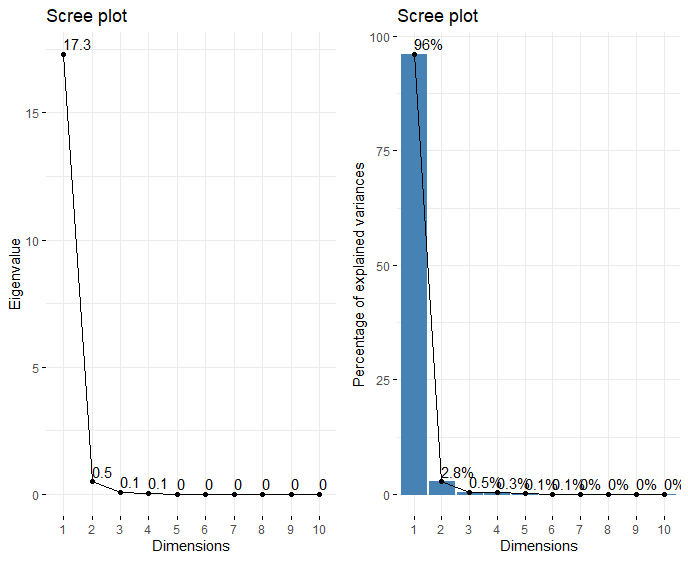
\includegraphics[width=1\linewidth]{images/Scree_plot_2_cul}
	\caption[Sơ đồ sàng lọc dữ liệu ca nhiễm hằng ngày và giá trị riêng tương ứng]{Sơ đồ sàng lọc cho kết quả đồ thị bên trái thể hiện giá trị riêng của từng thành phần chính. Trong đồ thị này, thành phần thứ nhất có giá trị riêng lớn nhất, thành phần thứ năm trở đi thì có giá trị riêng bé hơn $ 1 $. Sơ đồ bên phải thể hiện phần trăm phương sai được giải thích đối với từng thành phần. }
	\label{fig:screeplot2cul}
\end{figure}

Ở đây, thành phần chính đầu tiên đã giải thích một tỷ lệ rất lớn của phương sai, và các thành phần chính tiếp theo giải thích ít hơn nhiều. Điều này cho thấy chúng ta nên tập trung chủ yếu vào  thành phần chính thứ nhất. 




\newpage
\begin{Shaded}
	\begin{Highlighting}[]
\NormalTok{pca\_cul }\SpecialCharTok{\%\textgreater{}\%}\NormalTok{ factoextra}\SpecialCharTok{::}\FunctionTok{fviz\_pca\_biplot}\NormalTok{(.,}
		\AttributeTok{repel =} \ConstantTok{TRUE}\NormalTok{,}
		\AttributeTok{col.var =} \StringTok{"\#2E9FDF"}\NormalTok{,}
		\AttributeTok{col.ind =} \StringTok{"\#696969"}\NormalTok{)}
	\end{Highlighting}
\end{Shaded}

Tương tự đối với dữ liệu hằng ngày, ta nhìn rõ ràng hơn khi trực quan hóa vị trí của từng ngày được đánh số từ 1 đến 96 và biểu thị chỉ số cos2 bằng kích thước và phổ màu.
\begin{figure}[H]
	\centering
	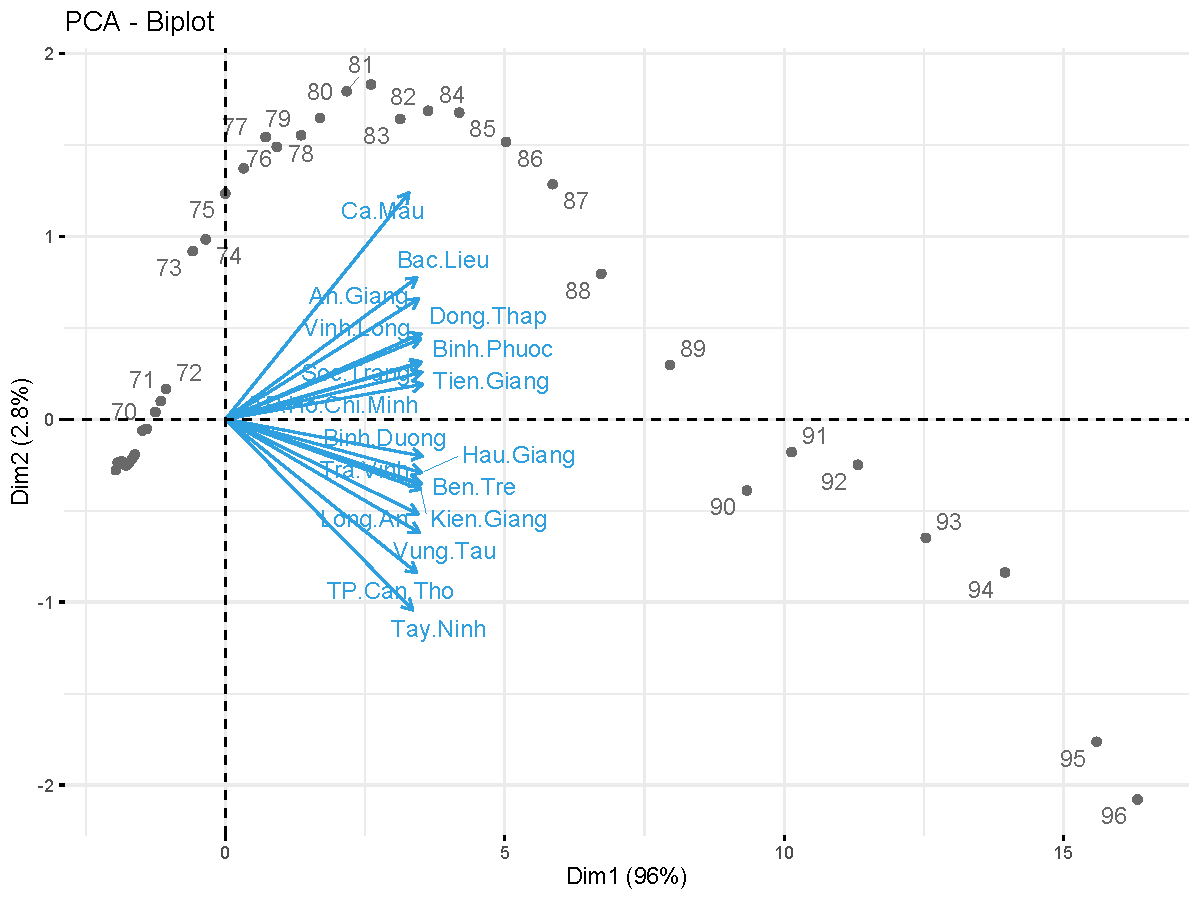
\includegraphics[width=0.75\linewidth]{images/biplot_cul}
	\caption[Biểu đồ biplot cho dữ liệu hằng ngày]{Biểu đồ biplot cho biết mối quan hệ giữa các biến ban đầu và các thành phần chính. Độ dài của vector cho biết độ mạnh của mối tương quan của biến ban đầu với thành phần chính.}
	\label{fig:biplotcul}
\end{figure}

\begin{Shaded}
	\begin{Highlighting}[]
\NormalTok{pca\_cul }\SpecialCharTok{\%\textgreater{}\%} \FunctionTok{fviz\_pca\_ind}\NormalTok{(.,}
		\AttributeTok{col.ind =} \StringTok{"cos2"}\NormalTok{,}
		\AttributeTok{pointsize =} \StringTok{"cos2"}\NormalTok{,}
		\AttributeTok{gradient.cols =} \FunctionTok{c}\NormalTok{(}\StringTok{"\#00AFBB"}\NormalTok{, }\StringTok{"\#E7B800"}\NormalTok{, }\StringTok{"\#FC4E07"}\NormalTok{),}
		\AttributeTok{repel =} \ConstantTok{TRUE}\NormalTok{) }
	\end{Highlighting}
\end{Shaded}


\begin{figure}[H]
	\centering
	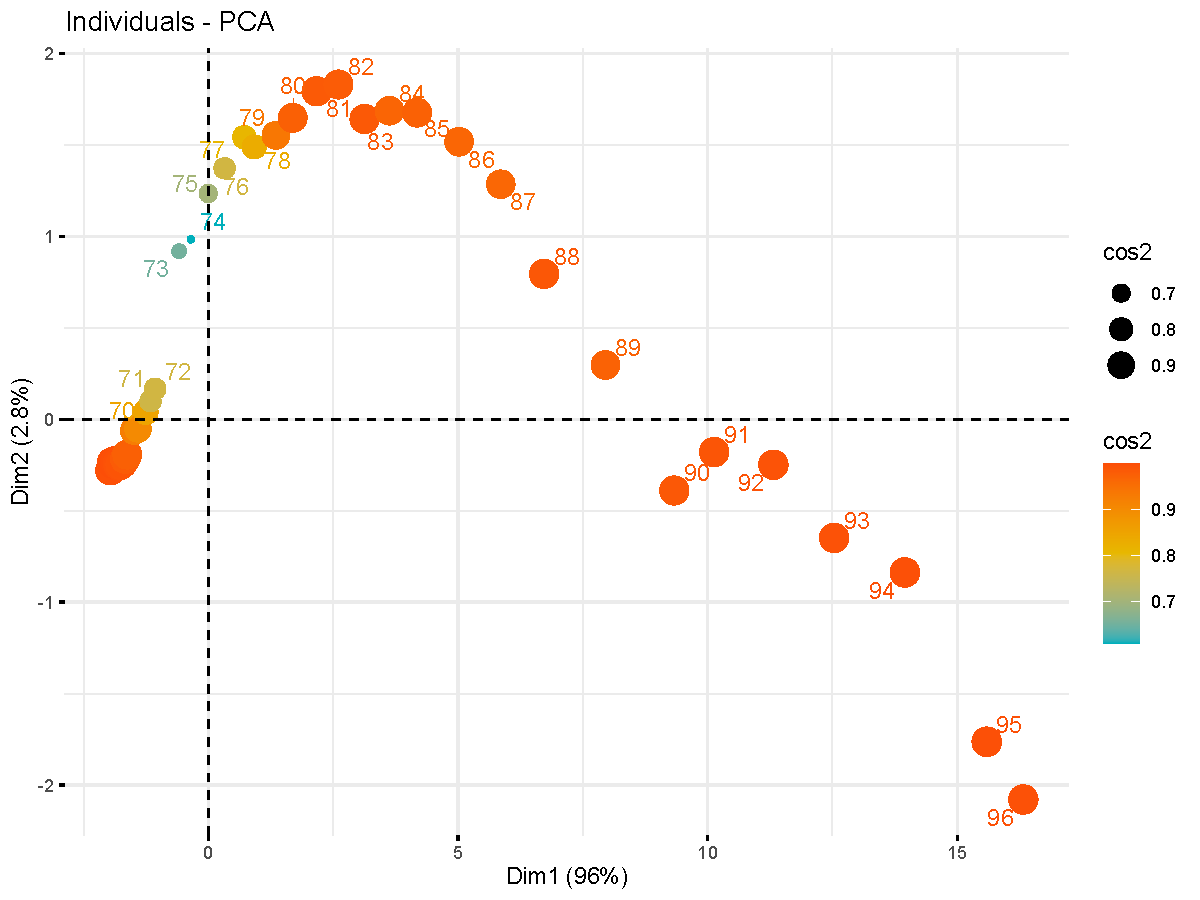
\includegraphics[width=0.75\linewidth]{images/ind_cul}
	\caption[Biểu đồ biplot tổng hợp mật độ cos2 giữa hai thành phần chính của dữ liệu tích lũy]{Biểu đồ biplot tổng hợp mật độ cos2 giữa hai thành phần chính của dữ liệu tích lũy. Biểu đồ giải thích chính xác hơn độ lớn của giá trị cos2 qua kích thước và phổ màu.}
	\label{fig:indcul}
\end{figure}

Không quá bất thường khi các véc-tơ biến dữ liệu tích lũy gần như có độ dài như sau do mối tương quan thuận đã phân tích phía trên.



\newpage
\begin{landscape}
	\begin{Shaded}
		\begin{Highlighting}[]
\NormalTok{pca\_cul }\SpecialCharTok{\%\textgreater{}\%}\NormalTok{ FactoMineR}\SpecialCharTok{::}\FunctionTok{plot.PCA}\NormalTok{(., }
		\AttributeTok{choix=}\StringTok{\textquotesingle{}var\textquotesingle{}}\NormalTok{,}
		\AttributeTok{select=}\StringTok{\textquotesingle{}contrib 5\textquotesingle{}}\NormalTok{)}
\NormalTok{pca\_cul }\SpecialCharTok{\%\textgreater{}\%}\NormalTok{ factoextra}\SpecialCharTok{::}\FunctionTok{fviz\_pca\_var}\NormalTok{(., }
		\AttributeTok{col.var =} \StringTok{"cos2"}\NormalTok{,}
		\AttributeTok{gradient.cols =} \FunctionTok{c}\NormalTok{(}\StringTok{"\#00AFBB"}\NormalTok{, }\StringTok{"\#E7B800"}\NormalTok{, }\StringTok{"\#FC4E07"}\NormalTok{), }
		\AttributeTok{repel =} \ConstantTok{TRUE}\NormalTok{)}
		\end{Highlighting}
	\end{Shaded}
	
	\begin{figure}[H]
		\centering
		\subfigure[Đồ thị biểu diễn tương quan theo hai chiều dữ liệu đầu tiên của dữ liệu tích lũy]{
			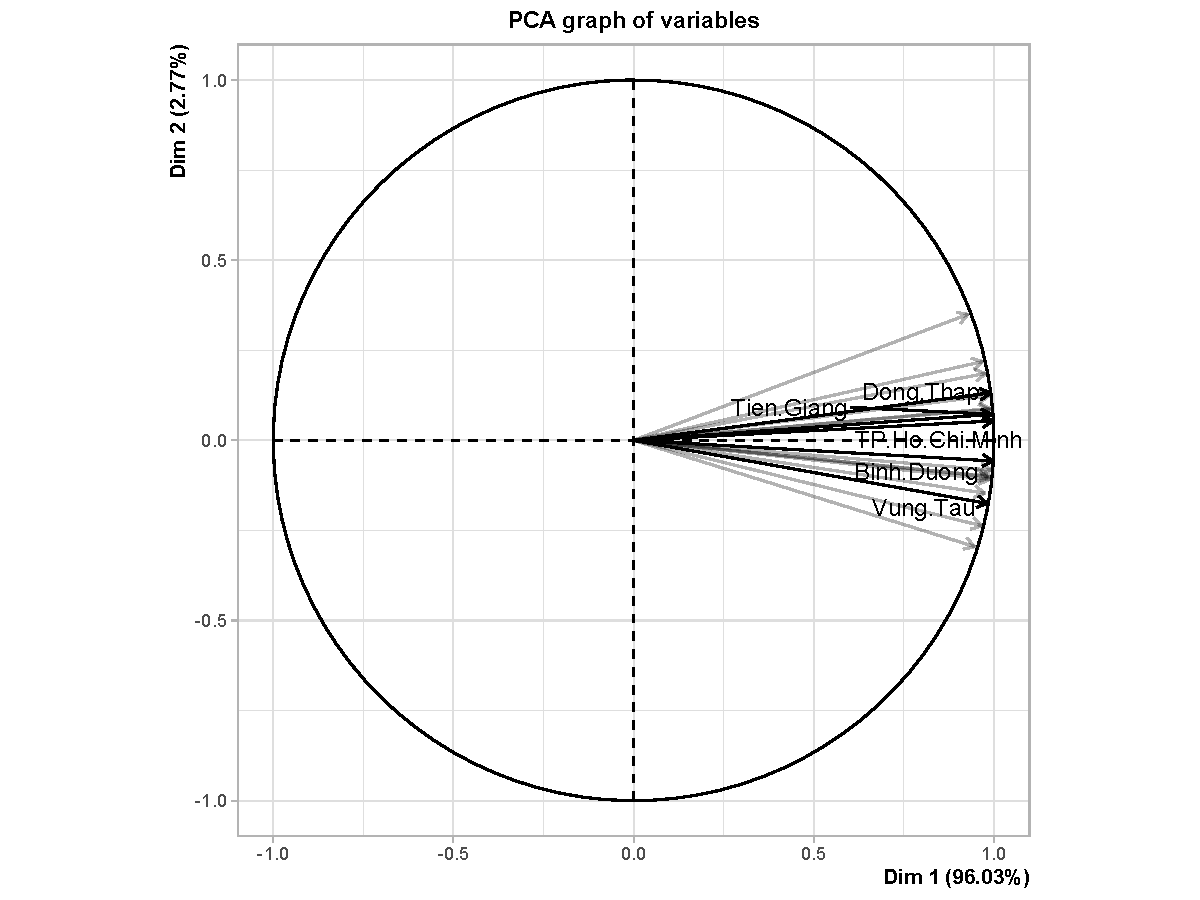
\includegraphics[width=0.48\linewidth]{images/contrib5_cul}		\label{fig:contrib5_cul}}
		\subfigure[Đồ thị biểu diễn cos2 của giá trị riêng theo hai chiều dữ liệu đầu tiên của dữ liệu tích lũy]{
			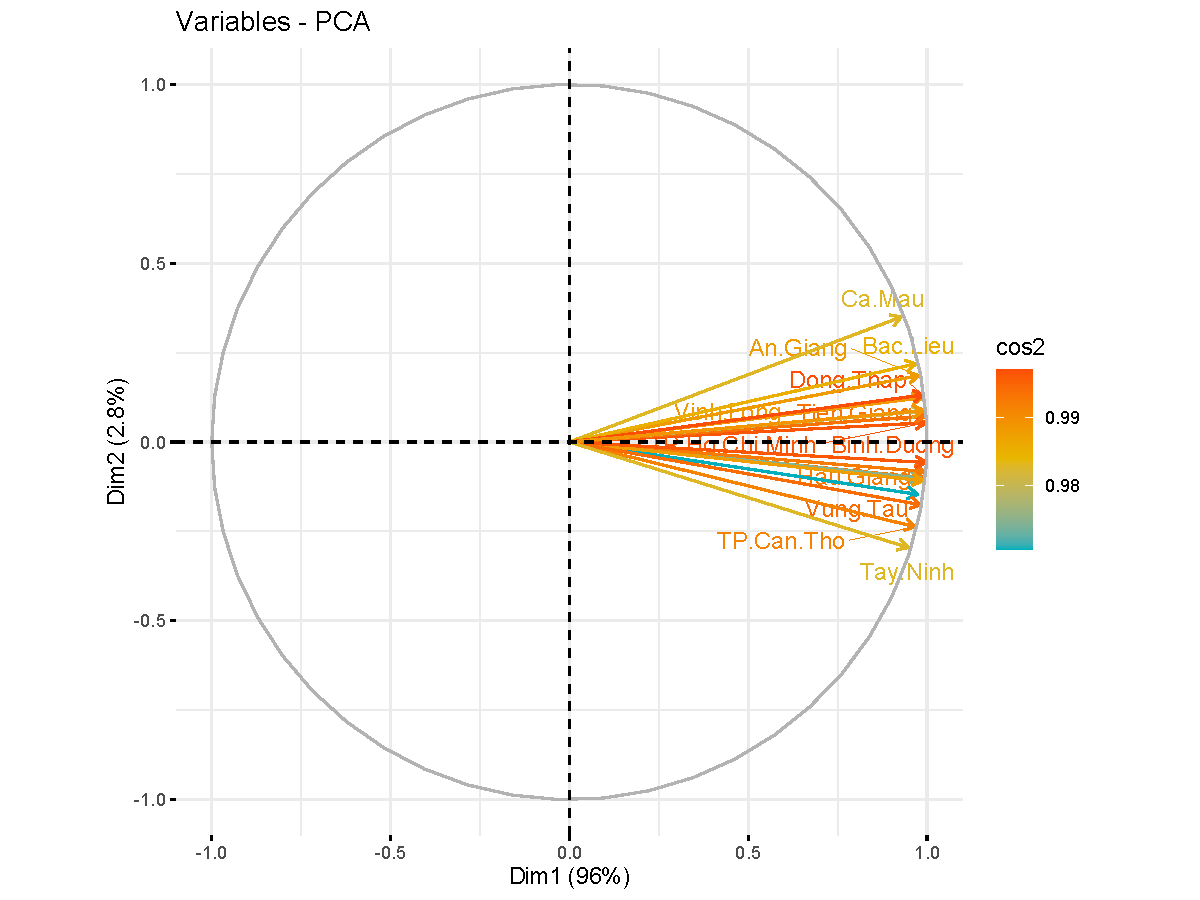
\includegraphics[width=0.48\linewidth]{images/circ_cos2_cul}		\label{fig:circcos2cul}}
		\caption[Đồ thị biểu diễn các thông số theo hai chiều đầu tiên với dữ liệu tích lũy]{Đồ thị biểu diễn các thông số theo hai chiều đầu tiên với dữ liệu tích lũy.}
	\end{figure}
Ta chia 5 biến được chọn thành hai nhóm. Nhóm 1 gồm hai tỉnh Đồng Tháp và Tiền Giang và Tp. Hồ Chí Minh; Nhóm 2 gồm hai tỉnh Bình Dương và Vũng Tàu.
\end{landscape}




\newpage
\begin{Shaded}
	\begin{Highlighting}[]
\NormalTok{factoextra}\SpecialCharTok{::}\FunctionTok{get\_eig}\NormalTok{(pca\_cul)}
	\end{Highlighting}
\end{Shaded}
\begin{verbatim}
##          eigenvalue variance.percent cumulative.variance.percent
## Dim.1  1.728623e+01     9.603460e+01                    96.03460
## Dim.2  4.979355e-01     2.766308e+00                    98.80091
## Dim.3  8.702444e-02     4.834691e-01                    99.28438
## Dim.4  5.914503e-02     3.285835e-01                    99.61296
## Dim.5  2.106883e-02     1.170491e-01                    99.73001
## Dim.6  1.725158e-02     9.584213e-02                    99.82585
## Dim.7  7.618441e-03     4.232467e-02                    99.86818
## Dim.8  6.073989e-03     3.374438e-02                    99.90192
## Dim.9  4.888367e-03     2.715759e-02                    99.92908
## Dim.10 4.301642e-03     2.389801e-02                    99.95298
## Dim.11 3.282633e-03     1.823685e-02                    99.97121
## Dim.12 1.923590e-03     1.068661e-02                    99.98190
## Dim.13 1.061794e-03     5.898857e-03                    99.98780
## Dim.14 8.760986e-04     4.867214e-03                    99.99267
## Dim.15 5.385863e-04     2.992146e-03                    99.99566
## Dim.16 4.952817e-04     2.751565e-03                    99.99841
## Dim.17 1.540549e-04     8.558604e-04                    99.99927
## Dim.18 1.320986e-04     7.338813e-04                   100.00000
\end{verbatim}




\begin{Shaded}
	\begin{Highlighting}[]
\FunctionTok{summary}\NormalTok{(pca\_cul)}
	\end{Highlighting}
\end{Shaded}

\begin{verbatim}
## 
## Call:
## FactoMineR::PCA(X = cul_data, graph = FALSE) 
## 
## 
## Eigenvalues
##                        Dim.1   Dim.2   Dim.3   Dim.4   Dim.5   Dim.6   Dim.7
## Variance              17.286   0.498   0.087   0.059   0.021   0.017   0.008
## % of var.             96.035   2.766   0.483   0.329   0.117   0.096   0.042
## Cumulative % of var.  96.035  98.801  99.284  99.613  99.730  99.826  99.868
##                        Dim.8   Dim.9  Dim.10  Dim.11  Dim.12  Dim.13  Dim.14
## Variance               0.006   0.005   0.004   0.003   0.002   0.001   0.001
## % of var.              0.034   0.027   0.024   0.018   0.011   0.006   0.005
## Cumulative % of var.  99.902  99.929  99.953  99.971  99.982  99.988  99.993
##                       Dim.15  Dim.16  Dim.17  Dim.18
## Variance               0.001   0.000   0.000   0.000
## % of var.              0.003   0.003   0.001   0.001
## Cumulative % of var.  99.996  99.998  99.999 100.000
## 
## Individuals (the 10 first)
##                    Dist    Dim.1    ctr   cos2    Dim.2    ctr   cos2    Dim.3
## 1              |  1.987 | -1.964  0.232  0.977 | -0.279  0.163  0.020 | -0.064
## 2              |  1.987 | -1.964  0.232  0.977 | -0.279  0.163  0.020 | -0.064
## 3              |  1.987 | -1.964  0.232  0.977 | -0.279  0.163  0.020 | -0.064
## 4              |  1.987 | -1.964  0.232  0.977 | -0.279  0.163  0.020 | -0.064
## 5              |  1.987 | -1.964  0.232  0.977 | -0.279  0.163  0.020 | -0.064
## 6              |  1.987 | -1.964  0.232  0.977 | -0.279  0.163  0.020 | -0.064
## 7              |  1.987 | -1.964  0.232  0.977 | -0.279  0.163  0.020 | -0.064
## 8              |  1.987 | -1.964  0.232  0.977 | -0.279  0.163  0.020 | -0.064
## 9              |  1.987 | -1.964  0.232  0.977 | -0.279  0.163  0.020 | -0.064
## 10             |  1.987 | -1.964  0.232  0.977 | -0.279  0.163  0.020 | -0.064
##                   ctr   cos2  
## 1               0.049  0.001 |
## 2               0.049  0.001 |
## 3               0.049  0.001 |
## 4               0.049  0.001 |
## 5               0.049  0.001 |
## 6               0.049  0.001 |
## 7               0.049  0.001 |
## 8               0.049  0.001 |
## 9               0.049  0.001 |
## 10              0.049  0.001 |
## 
## Variables (the 10 first)
##                   Dim.1    ctr   cos2    Dim.2    ctr   cos2    Dim.3    ctr
## TP.Ho.Chi.Minh |  0.997  5.748  0.994 |  0.054  0.581  0.003 | -0.033  1.247
## Tien.Giang     |  0.994  5.717  0.988 |  0.072  1.048  0.005 | -0.011  0.149
## Long.An        |  0.974  5.491  0.949 | -0.147  4.313  0.021 |  0.003  0.011
## An.Giang       |  0.977  5.518  0.954 |  0.186  6.922  0.034 |  0.081  7.603
## Ben.Tre        |  0.991  5.681  0.982 | -0.100  2.011  0.010 | -0.077  6.780
## TP.Can.Tho     |  0.967  5.410  0.935 | -0.237 11.300  0.056 |  0.031  1.105
## Vinh.Long      |  0.987  5.632  0.973 |  0.124  3.087  0.015 | -0.101 11.667
## Tra.Vinh       |  0.982  5.580  0.965 | -0.101  2.046  0.010 |  0.107 13.254
## Ca.Mau         |  0.928  4.979  0.861 |  0.350 24.550  0.122 |  0.090  9.246
## Hau.Giang      |  0.993  5.702  0.986 | -0.083  1.369  0.007 |  0.011  0.142
##                  cos2  
## TP.Ho.Chi.Minh  0.001 |
## Tien.Giang      0.000 |
## Long.An         0.000 |
## An.Giang        0.007 |
## Ben.Tre         0.006 |
## TP.Can.Tho      0.001 |
## Vinh.Long       0.010 |
## Tra.Vinh        0.012 |
## Ca.Mau          0.008 |
## Hau.Giang       0.000 |
\end{verbatim}


\newpage
Để thấy độ lớn của các cos2 trong các biến chính đã được chọn, ta có
\begin{Shaded}
	\begin{Highlighting}[]
\NormalTok{var }\OtherTok{\textless{}{-}}\NormalTok{ pca\_case }\SpecialCharTok{\%\textgreater{}\%}\NormalTok{ factoextra}\SpecialCharTok{::}\FunctionTok{get\_pca\_var}\NormalTok{()}
		\FunctionTok{corrplot}\NormalTok{(var}\SpecialCharTok{$}\NormalTok{cos2, }\AttributeTok{is.corr =} \ConstantTok{FALSE}\NormalTok{)}
\NormalTok{var }\OtherTok{\textless{}{-}}\NormalTok{ pca\_cul }\SpecialCharTok{\%\textgreater{}\%}\NormalTok{ factoextra}\SpecialCharTok{::}\FunctionTok{get\_pca\_var}\NormalTok{()}
		\FunctionTok{corrplot}\NormalTok{(var}\SpecialCharTok{$}\NormalTok{cos2, }\AttributeTok{is.corr =} \ConstantTok{FALSE}\NormalTok{)}
	\end{Highlighting}
\end{Shaded}

\begin{figure}[H]
	\centering
	\subfigure[Tương quan giữa các biến trong \textsf{cos2} của dữ liệu hằng ngày]{
		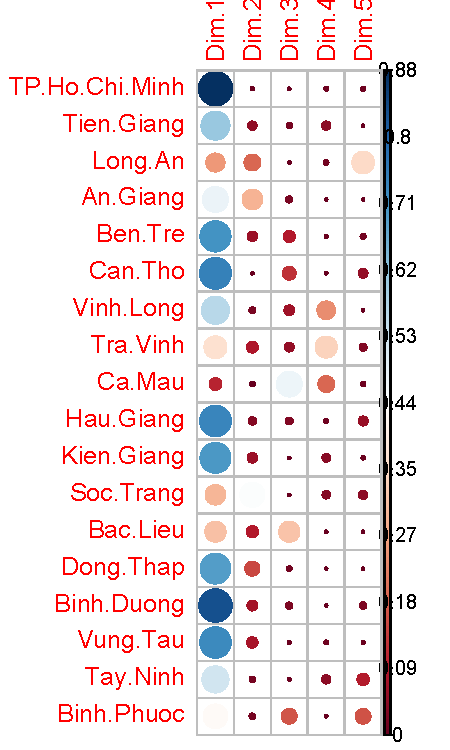
\includegraphics[width=0.65 \linewidth]{images/dimcase}		\label{fig:dimcase}}
	\subfigure[Tương quan giữa các biến trong \textsf{cos2} của dữ liệu tích lũy]{
		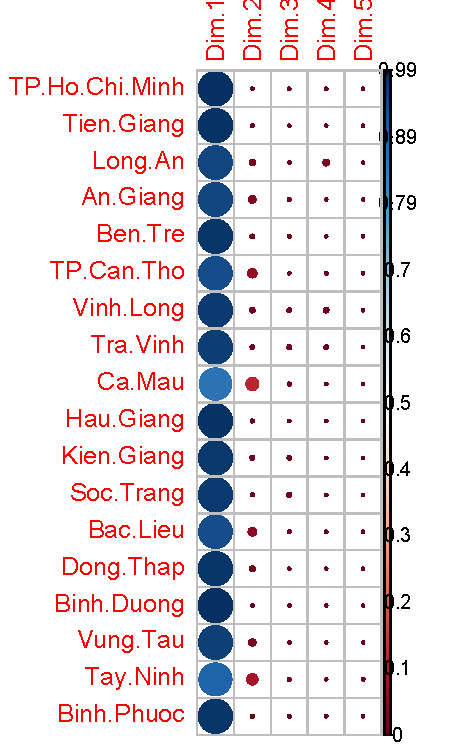
\includegraphics[width=0.65\linewidth]{images/dimcul}		\label{fig:dimcul}}
	\caption[Biểu đồ giá trị cos2 đối với 5 biến đã được chọn làm thành phần chính đối với các biến khi chưa phân tích.]{Biểu đồ giá trị cos2 đối với 5 biến đã được chọn làm thành phần chính đối với các biến khi chưa phân tích.}
\end{figure}































\newpage
\section{Kiểm định Bartlett -- KMO}

Tiến hành kiểm định Bartlett với dữ liệu \textsf{covid\_case} trong gói lệnh \textbf{psych}. Mục đích của kiểm định này là kiểm tra giả thiết các mẫu có phương sai bằng nhau 
\begin{Shaded}
	\begin{Highlighting}[]
\NormalTok{case\_data }\SpecialCharTok{\%\textgreater{}\%}\NormalTok{ psych}\SpecialCharTok{::}\FunctionTok{cortest.bartlett}\NormalTok{()}
	\end{Highlighting}
\end{Shaded}

\begin{verbatim}
	## R was not square, finding R from data
\end{verbatim}

\begin{verbatim}
	## $chisq
	## [1] 2105.383
	## 
	## $p.value
	## [1] 0
	## 
	## $df
	## [1] 153
\end{verbatim}

Ở đây, giá trị $ p-value = 0 $nhau, ta bác bỏ giả thiết phương sai bằng nhau từng đôi. Tức là dữ liệu thích hợp để phân tích nhân tố. Mặt khác ta cũng kiểm định KMO để xem 


\begin{Shaded}
	\begin{Highlighting}[]
\NormalTok{case\_data }\SpecialCharTok{\%\textgreater{}\%}\NormalTok{ psych}\SpecialCharTok{::}\FunctionTok{KMO}\NormalTok{()}
	\end{Highlighting}
\end{Shaded}

\begin{verbatim}
	## Kaiser-Meyer-Olkin factor adequacy
	## Call: psych::KMO(r = .)
	## Overall MSA =  0.77
	## MSA for each item = 
	## TP.Ho.Chi.Minh     Tien.Giang        Long.An       An.Giang        Ben.Tre 
	##           0.84           0.87           0.44           0.74           0.72 
	##        Can.Tho      Vinh.Long       Tra.Vinh         Ca.Mau      Hau.Giang 
	##           0.72           0.74           0.63           0.73           0.77 
	##     Kien.Giang      Soc.Trang       Bac.Lieu      Dong.Thap     Binh.Duong 
	##           0.77           0.63           0.79           0.87           0.90 
	##       Vung.Tau       Tay.Ninh     Binh.Phuoc 
	##           0.86           0.78           0.84
\end{verbatim}

Giá trị KMO trung bình nằm ở mức $ 0.77 $. Theo tiêu chuẩn đánh giá phù hợp để phân tích nhân tố, giá trị $ Overall MSA \geq 0.7 $, ta xác định dữ liệu rất thích hợp để phân tích nhân tố. Hệ số MSA của biến Long An dưới mức phù hợp ($ 0.44 $) nên khi phân tích nhân tố ta loại bỏ biến Long An. Sau khi tiến hành bỏ biến Long An trong dữ liệu thì $ Overall MSA $ có sự thay đổi

\begin{Shaded}
	\begin{Highlighting}[]
\NormalTok{case\_data }\SpecialCharTok{\%\textgreater{}\%} \FunctionTok{select}\NormalTok{(.,}\SpecialCharTok{{-}}\NormalTok{Long.An) }\SpecialCharTok{\%\textgreater{}\%} 
\FunctionTok{KMO}\NormalTok{() }\SpecialCharTok{\%\textgreater{}\%}\NormalTok{  .}\SpecialCharTok{\$}\NormalTok{MSA}
	\end{Highlighting}
\end{Shaded}

\begin{verbatim}
	## [1] 0.8227004
\end{verbatim}

Chỉ số $ MSA = 0.82 $ đã được cải thiện sau khi loại trừ biến Long An có $ MSA = 0.44 $ khá thấp và không phù hợp để phân tích nhân tố.


\newpage
Ta thực hiện kiểm định Barlett đối với dữ liệu tích lũy, với giả thiết thống kê 
\begin{Shaded}
	\begin{Highlighting}[]
\NormalTok{cul\_data }\SpecialCharTok{\%\textgreater{}\%}\NormalTok{ psych}\SpecialCharTok{::}\FunctionTok{cortest.bartlett}\NormalTok{()}
	\end{Highlighting}
\end{Shaded}

\begin{verbatim}
	## R was not square, finding R from data
\end{verbatim}

\begin{verbatim}
	## $chisq
	## [1] 7978.616
	## 
	## $p.value
	## [1] 0
	## 
	## $df
	## [1] 153
\end{verbatim}


Ở đây, giá trị $ p-value = 0 $ tức là bác bỏ giả thiết . Tức là dữ liệu cũng thích hợp để phân tích nhân tố. Mặt khác ta cũng kiểm định KMO để xem

\begin{Shaded}
	\begin{Highlighting}[]
\NormalTok{cul\_data }\SpecialCharTok{\%\textgreater{}\%}\NormalTok{ psych}\SpecialCharTok{::}\FunctionTok{KMO}\NormalTok{()}
	\end{Highlighting}
\end{Shaded}

\begin{verbatim}
	## Kaiser-Meyer-Olkin factor adequacy
	## Call: psych::KMO(r = .)
	## Overall MSA =  0.87
	## MSA for each item = 
	## TP.Ho.Chi.Minh     Tien.Giang        Long.An       An.Giang        Ben.Tre 
	##           0.89           0.85           0.83           0.84           0.84 
	##     TP.Can.Tho      Vinh.Long       Tra.Vinh         Ca.Mau      Hau.Giang 
	##           0.83           0.94           0.85           0.95           0.85 
	##     Kien.Giang      Soc.Trang       Bac.Lieu      Dong.Thap     Binh.Duong 
	##           0.84           0.87           0.94           0.87           0.87 
	##       Vung.Tau       Tay.Ninh     Binh.Phuoc 
	##           0.93           0.84           0.94
\end{verbatim}

Giá trị KMO trung bình nằm ở mức $ 0.87 $ sự thích hợp để phân tích nhân tố là rất cao. Như vậy bảng dữ liệu đủ điều kiện để phân tích nhân tố. Tất cả các biến đều có giá trị MSA trên $ 0.6 $ nên ta không cần loại biến nào. Cả hai dữ liệu trên đều sẵn sàng để phân tích nhân tố.

Đối với dữ liệu hằng ngày, ta chọn số nhân tố là 3 và đối với dữ liệu tích lũy ta chọn 2 nhân tố. Vì dữ liệu có 96 quan sát nên ta chọn hệ số tải (Factor Loading) là $ 0.55 $

Như đã phân tích, biến Long An trong dữ liệu hằng ngày có $ KMO $ thấp nên được loại khỏi dữ liệu 







\newpage

\section{Phân tích nhân tố}

\begin{Shaded}
	\begin{Highlighting}[]
\FunctionTok{principal}\NormalTok{(case\_data }\SpecialCharTok{\%\textgreater{}\%} \FunctionTok{select}\NormalTok{(}\SpecialCharTok{{-}}\NormalTok{Long.An), }
		\AttributeTok{nfactors =} \FloatTok{3}
		\AttributeTok{rotate =} \StringTok{"varimax"}\NormalTok{) }\SpecialCharTok{\%\textgreater{}\%} 
	\FunctionTok{print.psych}\NormalTok{(., }
		\AttributeTok{cut =} \FloatTok{0.55}\NormalTok{, }
		\AttributeTok{sort =} \ConstantTok{TRUE}\NormalTok{)}
	\end{Highlighting}
\end{Shaded}

\begin{verbatim}
## Principal Components Analysis
## Call: principal(r = case_data %>% select(-Long.An), nfactors = Nfacs, 
##     rotate = "varimax")
## Standardized loadings (pattern matrix) based upon correlation matrix
##                item   RC1   RC2   RC3   h2    u2 com
## Binh.Duong       14  0.92             0.94 0.055 1.2
## Hau.Giang         9  0.86             0.82 0.176 1.3
## Can.Tho           5  0.85             0.88 0.117 1.4
## Vung.Tau         15  0.84             0.82 0.185 1.3
## Kien.Giang       10  0.80             0.77 0.229 1.4
## Tien.Giang        2  0.76             0.67 0.334 1.3
## TP.Ho.Chi.Minh    1  0.66  0.57       0.89 0.108 2.5
## Tay.Ninh         16  0.65             0.54 0.460 1.6
## Soc.Trang        11        0.85       0.74 0.257 1.0
## An.Giang          3        0.83       0.81 0.192 1.4
## Dong.Thap        13        0.76       0.85 0.146 2.0
## Ben.Tre           4  0.63  0.69       0.87 0.135 2.0
## Tra.Vinh          7        0.55       0.51 0.492 1.9
## Vinh.Long         6                   0.65 0.347 3.0
## Bac.Lieu         12              0.77 0.73 0.272 1.4
## Ca.Mau            8              0.74 0.59 0.415 1.1
## Binh.Phuoc       17              0.63 0.64 0.359 2.0
## 
##                        RC1  RC2  RC3
## SS loadings           6.43 3.87 2.42
## Proportion Var        0.38 0.23 0.14
## Cumulative Var        0.38 0.61 0.75
## Proportion Explained  0.51 0.30 0.19
## Cumulative Proportion 0.51 0.81 1.00
## 
## Mean item complexity =  1.6
## Test of the hypothesis that 3 components are sufficient.
## 
## The root mean square of the residuals (RMSR) is  0.07 
##  with the empirical chi square  117.62  with prob <  0.019 
## 
## Fit based upon off diagonal values = 0.99
\end{verbatim}


\begin{Shaded}
	\begin{Highlighting}[]
\FunctionTok{principal}\NormalTok{(cul\_data, }
		\AttributeTok{nfactors =} \DecValTok{1}\NormalTok{, }
		\AttributeTok{rotate =} \StringTok{"varimax"}\NormalTok{) }\SpecialCharTok{\%\textgreater{}\%} 
	\FunctionTok{print.psych}\NormalTok{(., }
		\AttributeTok{cut =} \FloatTok{0.55}\NormalTok{, }
		\AttributeTok{sort =} \ConstantTok{TRUE}\NormalTok{)}
	\end{Highlighting}
\end{Shaded}

\begin{verbatim}
## Principal Components Analysis
## Call: principal(r = cul_data, nfactors = 1, rotate = "varimax")
## Standardized loadings (pattern matrix) based upon correlation matrix
##                 V  PC1   h2     u2 com
## TP.Ho.Chi.Minh  1 1.00 0.99 0.0064   1
## Binh.Duong     15 1.00 0.99 0.0070   1
## Tien.Giang      2 0.99 0.99 0.0118   1
## Hau.Giang      10 0.99 0.99 0.0144   1
## Ben.Tre         5 0.99 0.98 0.0180   1
## Binh.Phuoc     18 0.99 0.98 0.0189   1
## Dong.Thap      14 0.99 0.98 0.0202   1
## Kien.Giang     11 0.99 0.98 0.0241   1
## Vinh.Long       7 0.99 0.97 0.0265   1
## Soc.Trang      12 0.99 0.97 0.0265   1
## Tra.Vinh        8 0.98 0.96 0.0355   1
## Vung.Tau       16 0.98 0.96 0.0366   1
## An.Giang        4 0.98 0.95 0.0462   1
## Long.An         3 0.97 0.95 0.0509   1
## Bac.Lieu       13 0.97 0.94 0.0625   1
## TP.Can.Tho      6 0.97 0.94 0.0649   1
## Tay.Ninh       17 0.95 0.90 0.1041   1
## Ca.Mau          9 0.93 0.86 0.1394   1
## 
##                  PC1
## SS loadings    17.29
## Proportion Var  0.96
## 
## Mean item complexity =  1
## Test of the hypothesis that 1 component is sufficient.
## 
## The root mean square of the residuals (RMSR) is  0.03 
##  with the empirical chi square  20.23  with prob <  1 
## 
## Fit based upon off diagonal values = 1
\end{verbatim}


\newpage

\section{Ma trận xoay}
\begin{Shaded}
	\begin{Highlighting}[]
\NormalTok{fa\_case }\OtherTok{\textless{}{-}}\NormalTok{ case\_data }\SpecialCharTok{\%\textgreater{}\%} \FunctionTok{select}\NormalTok{(}\SpecialCharTok{{-}}\NormalTok{Long.An) }\SpecialCharTok{\%\textgreater{}\%}
	\FunctionTok{factanal}\NormalTok{(., }\DecValTok{3}\NormalTok{, }
		\AttributeTok{rotation =} \StringTok{"varimax"}\NormalTok{)}		
\NormalTok{fa\_cul }\OtherTok{\textless{}{-}}\NormalTok{ cul\_data }\SpecialCharTok{\%\textgreater{}\%} \FunctionTok{factanal}\NormalTok{(., }\DecValTok{2}\NormalTok{, }
		\AttributeTok{rotation =} \StringTok{"varimax"}\NormalTok{)}
\FunctionTok{fa.diagram}\NormalTok{(fa\_case}\SpecialCharTok{$}\NormalTok{loadings)}
\FunctionTok{fa.diagram}\NormalTok{(fa\_cul}\SpecialCharTok{$}\NormalTok{loadings)}
	\end{Highlighting}
\end{Shaded}

\begin{figure}[H]
	\centering
	\subfigure[Nhân tố dữ liệu hằng ngày]{
		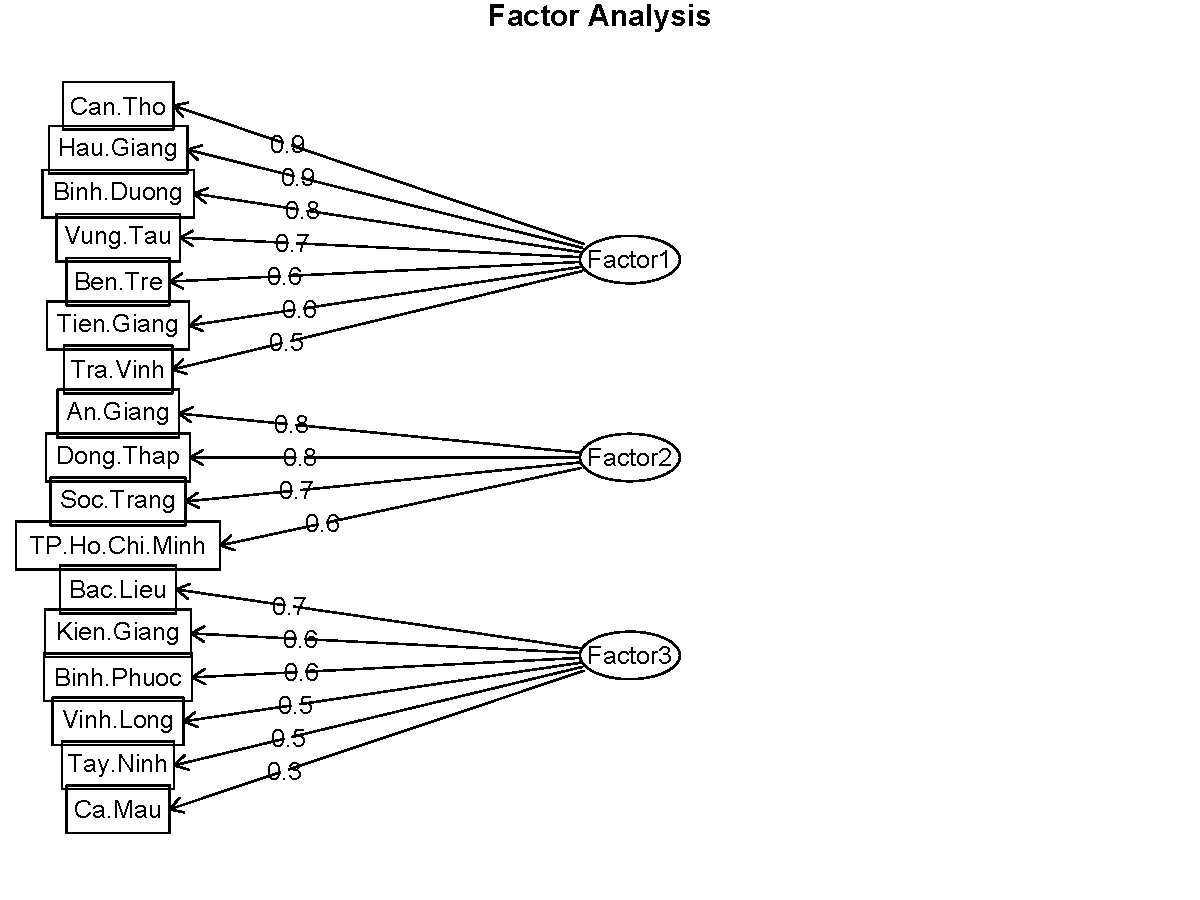
\includegraphics[width=0.7 \linewidth]{images/fa_case}		\label{fig:facase}}
	\subfigure[Nhân tố dữ liệu tích lũy]{
		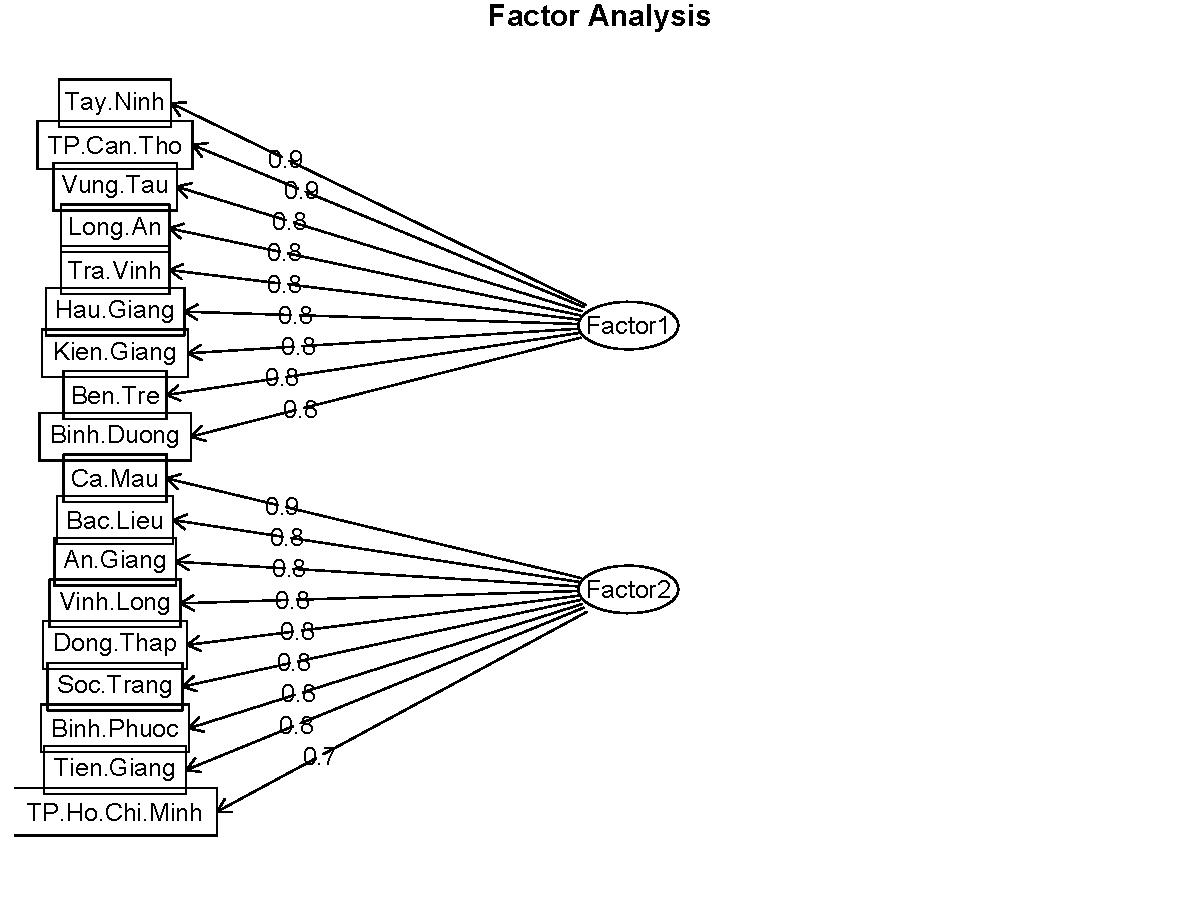
\includegraphics[width=0.7  \linewidth]{images/fa_cul}		\label{fig:facul}}
	\caption[Phân cụm nhân tố và hệ số nhân tố tương ứng của hai dữ liệu.]{Phân cum nhân tố và hệ số nhân tố tương ứng của hai dữ liệu.}
\end{figure} 



\begin{Shaded}
	\begin{Highlighting}[]
\NormalTok{fa\_case }\SpecialCharTok{\%\textgreater{}\%} \FunctionTok{factor.plot}\NormalTok{(., }\AttributeTok{cut =} \FloatTok{0.55}\NormalTok{)}
\NormalTok{fa\_cul }\SpecialCharTok{\%\textgreater{}\%} \FunctionTok{factor.plot}\NormalTok{(., }\AttributeTok{cut =} \FloatTok{0.55}\NormalTok{)}
	\end{Highlighting}
\end{Shaded}

\begin{figure}[H]
	\centering
	\subfigure[Tương quan nhân tố của dữ liệu hằng ngày. Với ba nhân tố được xác định với hệ số tải nhân tố $ 0.55 $]{
		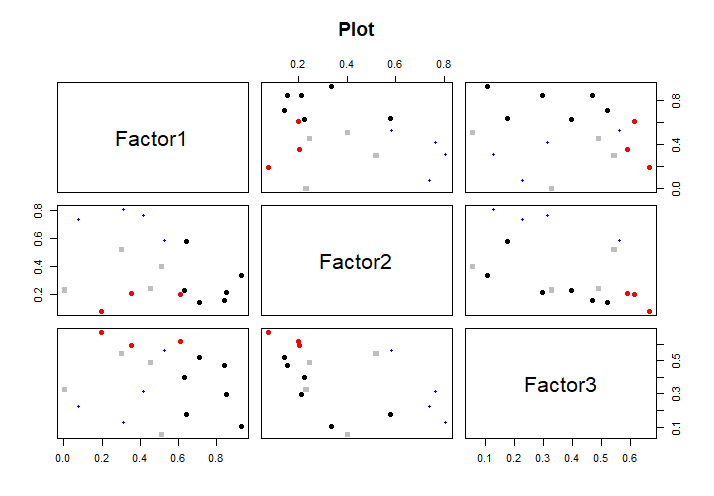
\includegraphics[width=0.77 \linewidth]{images/fa_case3}		\label{fig:facase3}}
	\subfigure[Tương quan nhân tố của dữ liệu tích lũy. Với hai nhân tố được xác định với hệ số tải nhân tố $ 0.55 $]{
		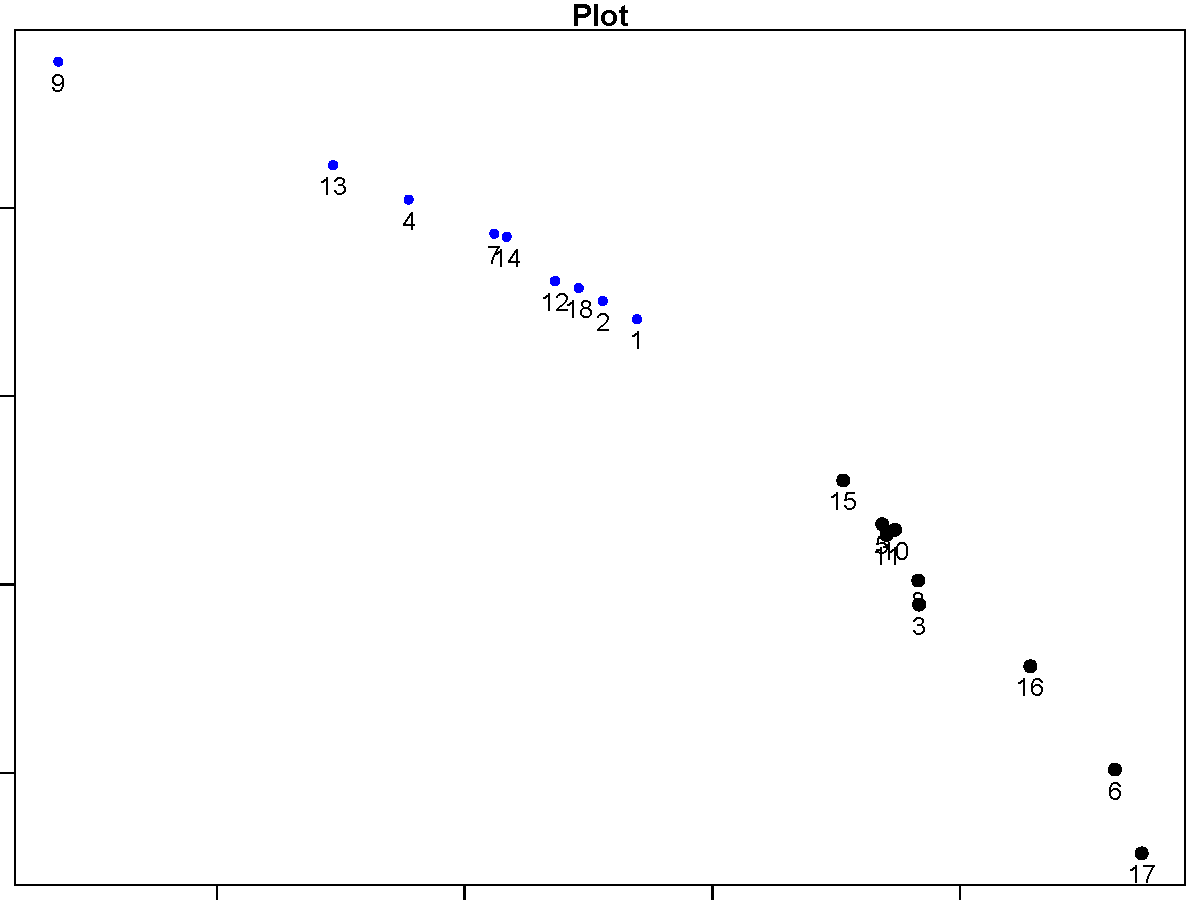
\includegraphics[width=0.65\linewidth]{images/fa_cul2}		\label{fig:facul2}}
	\caption[Tương quan nhân tố của dữ liệu nhân tố được xác định với hệ số tải nhân tố $ 0.55 $]{Tương quan nhân tố của dữ liệu nhân tố được xác định với hệ số tải nhân tố $ 0.55 $}
\end{figure}


\newpage
\section{Bàn luận}
Do các tác động xã hội, kinh tế và môi trường khác nhau của Covid-19, điều quan trọng là phải nghiên cứu và so sánh tốc độ lây lan của bệnh này ở các tỉnh/thành phố khác nhau. Trong nghiên cứu này, số lượng bệnh nhân có Covid-19 ở 18 tỉnh/thành phố đã được xem xét. Đầu tiên, mối quan hệ giữa các tỉnh/thành phố được xem xét được nghiên cứu bằng cách sử dụng mối tương quan của Pearson. Kết quả chỉ ra rằng có mối quan hệ thuận chiều cực kỳ cao giữa các tỉnh/thành phố được xem xét, dựa trên số lượng bệnh nhân mắc bệnh Covid-19 và tích lũy của số ca nhiễm bệnh theo ngày. Sau đó, dựa trên tốc độ lây lan của Covid-19, các tỉnh/thành phố này được phân loại bằng cách sử dụng phân tích thành phần chính. Kết quả chỉ ra rằng, đối với số lượng bệnh nhân, sự phân bố lây lan ở Sóc Trăng, An Giang, Trà Vinh, Đồng Tháp, Bến Tre, Vĩnh Long và Tp. Hồ Chí Minh là tương tự nhau và khác với các tỉnh/thành phố khác. Ngoài ra, đối với số lượng bệnh nhân tích lũy theo ngày, sự phân bố lây lan ở Bình Dương và Vũng Tàu là tương tự nhau và khác với các tỉnh Đồng Tháp, Tiền Giang và Tp. Hồ Chí Minh khi ta phân tích và chọn ra 5 thành phần chính tiêu biểu. Các tác giả đề nghị các nhà nghiên cứu xem xét nhiều tỉnh/thành phố hơn và phân loại chúng dựa trên phân tích thành phần chính hoặc các phương pháp khác như phân tích nhân tố có sự cải tiến.


\end{document}